\documentclass[a4paper]{book}
\usepackage{makeidx}
\usepackage{natbib}
\usepackage{graphicx}
\usepackage{multicol}
\usepackage{float}
\usepackage{listings}
\usepackage{color}
\usepackage{ifthen}
\usepackage[table]{xcolor}
\usepackage{textcomp}
\usepackage{alltt}
\usepackage{ifpdf}
\ifpdf
\usepackage[pdftex,
            pagebackref=true,
            colorlinks=true,
            linkcolor=blue,
            unicode
           ]{hyperref}
\else
\usepackage[ps2pdf,
            pagebackref=true,
            colorlinks=true,
            linkcolor=blue,
            unicode
           ]{hyperref}
\usepackage{pspicture}
\fi
\usepackage[utf8]{inputenc}
\usepackage{mathptmx}
\usepackage[scaled=.90]{helvet}
\usepackage{courier}
\usepackage{sectsty}
\usepackage[titles]{tocloft}
\usepackage{doxygen}
\lstset{language=C++,inputencoding=utf8,basicstyle=\footnotesize,breaklines=true,breakatwhitespace=true,tabsize=8,numbers=left }
\makeindex
\setcounter{tocdepth}{3}
\renewcommand{\footrulewidth}{0.4pt}
\renewcommand{\familydefault}{\sfdefault}
\hfuzz=15pt
\setlength{\emergencystretch}{15pt}
\hbadness=750
\tolerance=750
\begin{document}
\hypersetup{pageanchor=false,citecolor=blue}
\begin{titlepage}
\vspace*{7cm}
\begin{center}
{\Large \-J\-Spider \-Library }\\
\vspace*{1cm}
{\large \-Generated by Doxygen 1.7.6.1}\\
\vspace*{0.5cm}
{\small Thu Feb 16 2012 02:56:14}\\
\end{center}
\end{titlepage}
\clearemptydoublepage
\pagenumbering{roman}
\tableofcontents
\clearemptydoublepage
\pagenumbering{arabic}
\hypersetup{pageanchor=true,citecolor=blue}
\chapter{\-Namespace \-Index}
\section{\-Packages}
\-Here are the packages with brief descriptions (if available)\-:\begin{DoxyCompactList}
\item\contentsline{section}{\hyperlink{namespacecom}{com} }{\pageref{namespacecom}}{}
\item\contentsline{section}{\hyperlink{namespacecom_1_1spider}{com\-::spider} }{\pageref{namespacecom_1_1spider}}{}
\item\contentsline{section}{\hyperlink{namespacecom_1_1spider_1_1jspiderlibrary2}{com.\-spider.\-jspiderlibrary2} }{\pageref{namespacecom_1_1spider_1_1jspiderlibrary2}}{}
\end{DoxyCompactList}

\chapter{\-Class \-Index}
\section{\-Class \-Hierarchy}
\-This inheritance list is sorted roughly, but not completely, alphabetically\-:\begin{DoxyCompactList}
\item \contentsline{section}{com.\-spider.\-jspiderlibrary2.\-App\-Test}{\pageref{classcom_1_1spider_1_1jspiderlibrary2_1_1_app_test}}{}
\item \contentsline{section}{com.\-spider.\-jspiderlibrary2.\-H\-T\-M\-L\-Parse}{\pageref{classcom_1_1spider_1_1jspiderlibrary2_1_1_h_t_m_l_parse}}{}
\item \contentsline{section}{com.\-spider.\-jspiderlibrary2.\-I\-Spider\-Reportable}{\pageref{interfacecom_1_1spider_1_1jspiderlibrary2_1_1_i_spider_reportable}}{}
\begin{DoxyCompactList}
\item \contentsline{section}{com.\-spider.\-jspiderlibrary2.\-Communicator}{\pageref{classcom_1_1spider_1_1jspiderlibrary2_1_1_communicator}}{}
\end{DoxyCompactList}
\item \contentsline{section}{com.\-spider.\-jspiderlibrary2.\-Spider.\-Parser}{\pageref{classcom_1_1spider_1_1jspiderlibrary2_1_1_spider_1_1_parser}}{}
\item \contentsline{section}{com.\-spider.\-jspiderlibrary2.\-Robots\-Parser}{\pageref{classcom_1_1spider_1_1jspiderlibrary2_1_1_robots_parser}}{}
\item \contentsline{section}{com.\-spider.\-jspiderlibrary2.\-Spider}{\pageref{classcom_1_1spider_1_1jspiderlibrary2_1_1_spider}}{}
\end{DoxyCompactList}

\chapter{\-Class \-Index}
\section{\-Class \-List}
\-Here are the classes, structs, unions and interfaces with brief descriptions\-:\begin{DoxyCompactList}
\item\contentsline{section}{\hyperlink{classcom_1_1utn_1_1searchengine_1_1_app_test}{com.\-utn.\-searchengine.\-App\-Test} }{\pageref{classcom_1_1utn_1_1searchengine_1_1_app_test}}{}
\item\contentsline{section}{\hyperlink{classcom_1_1utn_1_1searchengine_1_1_local_word_count_manager_1_1_compare}{com.\-utn.\-searchengine.\-Local\-Word\-Count\-Manager.\-Compare} }{\pageref{classcom_1_1utn_1_1searchengine_1_1_local_word_count_manager_1_1_compare}}{}
\item\contentsline{section}{\hyperlink{classdataaccess_1_1factories_1_1_d_a_o_factory}{dataaccess.\-factories.\-D\-A\-O\-Factory} }{\pageref{classdataaccess_1_1factories_1_1_d_a_o_factory}}{}
\item\contentsline{section}{\hyperlink{classcom_1_1utn_1_1searchengine_1_1_document}{com.\-utn.\-searchengine.\-Document} }{\pageref{classcom_1_1utn_1_1searchengine_1_1_document}}{}
\item\contentsline{section}{\hyperlink{interfacedataaccess_1_1dao_1_1_document_d_a_o}{dataaccess.\-dao.\-Document\-D\-A\-O} }{\pageref{interfacedataaccess_1_1dao_1_1_document_d_a_o}}{}
\item\contentsline{section}{\hyperlink{classcom_1_1utn_1_1searchengine_1_1_document_manager}{com.\-utn.\-searchengine.\-Document\-Manager} }{\pageref{classcom_1_1utn_1_1searchengine_1_1_document_manager}}{}
\item\contentsline{section}{\hyperlink{classcom_1_1utn_1_1searchengine_1_1_document_results}{com.\-utn.\-searchengine.\-Document\-Results} }{\pageref{classcom_1_1utn_1_1searchengine_1_1_document_results}}{}
\item\contentsline{section}{\hyperlink{classcom_1_1utn_1_1searchengine_1_1_local_word_count_manager}{com.\-utn.\-searchengine.\-Local\-Word\-Count\-Manager} }{\pageref{classcom_1_1utn_1_1searchengine_1_1_local_word_count_manager}}{}
\item\contentsline{section}{\hyperlink{classdataaccess_1_1dbmanager_1_1_postgre_d_b_manager}{dataaccess.\-dbmanager.\-Postgre\-D\-B\-Manager} }{\pageref{classdataaccess_1_1dbmanager_1_1_postgre_d_b_manager}}{}
\item\contentsline{section}{\hyperlink{classdataaccess_1_1factories_1_1_postgre_s_q_l_d_a_o_factory}{dataaccess.\-factories.\-Postgre\-S\-Q\-L\-D\-A\-O\-Factory} }{\pageref{classdataaccess_1_1factories_1_1_postgre_s_q_l_d_a_o_factory}}{}
\item\contentsline{section}{\hyperlink{classdataaccess_1_1postgresql_1_1_postgre_s_q_l_document_d_a_o}{dataaccess.\-postgresql.\-Postgre\-S\-Q\-L\-Document\-D\-A\-O} }{\pageref{classdataaccess_1_1postgresql_1_1_postgre_s_q_l_document_d_a_o}}{}
\item\contentsline{section}{\hyperlink{classdataaccess_1_1postgresql_1_1_postgre_s_q_l_post_list_d_a_o}{dataaccess.\-postgresql.\-Postgre\-S\-Q\-L\-Post\-List\-D\-A\-O} }{\pageref{classdataaccess_1_1postgresql_1_1_postgre_s_q_l_post_list_d_a_o}}{}
\item\contentsline{section}{\hyperlink{classdataaccess_1_1postgresql_1_1_postgre_s_q_l_word_d_a_o}{dataaccess.\-postgresql.\-Postgre\-S\-Q\-L\-Word\-D\-A\-O} }{\pageref{classdataaccess_1_1postgresql_1_1_postgre_s_q_l_word_d_a_o}}{}
\item\contentsline{section}{\hyperlink{classcom_1_1utn_1_1searchengine_1_1_post_list}{com.\-utn.\-searchengine.\-Post\-List} }{\pageref{classcom_1_1utn_1_1searchengine_1_1_post_list}}{}
\item\contentsline{section}{\hyperlink{interfacedataaccess_1_1dao_1_1_post_list_d_a_o}{dataaccess.\-dao.\-Post\-List\-D\-A\-O} }{\pageref{interfacedataaccess_1_1dao_1_1_post_list_d_a_o}}{}
\item\contentsline{section}{\hyperlink{classcom_1_1utn_1_1searchengine_1_1_similitude}{com.\-utn.\-searchengine.\-Similitude} }{\pageref{classcom_1_1utn_1_1searchengine_1_1_similitude}}{}
\item\contentsline{section}{\hyperlink{classcom_1_1utn_1_1searchengine_1_1_stop_word_map}{com.\-utn.\-searchengine.\-Stop\-Word\-Map} }{\pageref{classcom_1_1utn_1_1searchengine_1_1_stop_word_map}}{}
\item\contentsline{section}{\hyperlink{classcom_1_1utn_1_1searchengine_1_1_vocabulary}{com.\-utn.\-searchengine.\-Vocabulary} }{\pageref{classcom_1_1utn_1_1searchengine_1_1_vocabulary}}{}
\item\contentsline{section}{\hyperlink{classcom_1_1utn_1_1searchengine_1_1_word}{com.\-utn.\-searchengine.\-Word} }{\pageref{classcom_1_1utn_1_1searchengine_1_1_word}}{}
\item\contentsline{section}{\hyperlink{classcom_1_1utn_1_1searchengine_1_1_word_count}{com.\-utn.\-searchengine.\-Word\-Count} }{\pageref{classcom_1_1utn_1_1searchengine_1_1_word_count}}{}
\item\contentsline{section}{\hyperlink{interfacedataaccess_1_1dao_1_1_word_d_a_o}{dataaccess.\-dao.\-Word\-D\-A\-O} }{\pageref{interfacedataaccess_1_1dao_1_1_word_d_a_o}}{}
\item\contentsline{section}{\hyperlink{classcom_1_1utn_1_1searchengine_1_1_word_tracker}{com.\-utn.\-searchengine.\-Word\-Tracker} }{\pageref{classcom_1_1utn_1_1searchengine_1_1_word_tracker}}{}
\end{DoxyCompactList}

\chapter{\-File \-Index}
\section{\-File \-List}
\-Here is a list of all files with brief descriptions\-:\begin{DoxyCompactList}
\item\contentsline{section}{src/main/java/com/utn/searchengine/\hyperlink{_document_8java}{\-Document.\-java} }{\pageref{_document_8java}}{}
\item\contentsline{section}{src/main/java/com/utn/searchengine/\hyperlink{_document_manager_8java}{\-Document\-Manager.\-java} }{\pageref{_document_manager_8java}}{}
\item\contentsline{section}{src/main/java/com/utn/searchengine/\hyperlink{_document_results_8java}{\-Document\-Results.\-java} }{\pageref{_document_results_8java}}{}
\item\contentsline{section}{src/main/java/com/utn/searchengine/\hyperlink{_local_word_count_manager_8java}{\-Local\-Word\-Count\-Manager.\-java} }{\pageref{_local_word_count_manager_8java}}{}
\item\contentsline{section}{src/main/java/com/utn/searchengine/\hyperlink{_post_list_8java}{\-Post\-List.\-java} }{\pageref{_post_list_8java}}{}
\item\contentsline{section}{src/main/java/com/utn/searchengine/\hyperlink{_similitude_8java}{\-Similitude.\-java} }{\pageref{_similitude_8java}}{}
\item\contentsline{section}{src/main/java/com/utn/searchengine/\hyperlink{_stop_word_map_8java}{\-Stop\-Word\-Map.\-java} }{\pageref{_stop_word_map_8java}}{}
\item\contentsline{section}{src/main/java/com/utn/searchengine/\hyperlink{_vocabulary_8java}{\-Vocabulary.\-java} }{\pageref{_vocabulary_8java}}{}
\item\contentsline{section}{src/main/java/com/utn/searchengine/\hyperlink{_word_8java}{\-Word.\-java} }{\pageref{_word_8java}}{}
\item\contentsline{section}{src/main/java/com/utn/searchengine/\hyperlink{_word_count_8java}{\-Word\-Count.\-java} }{\pageref{_word_count_8java}}{}
\item\contentsline{section}{src/main/java/com/utn/searchengine/\hyperlink{_word_tracker_8java}{\-Word\-Tracker.\-java} }{\pageref{_word_tracker_8java}}{}
\item\contentsline{section}{src/main/java/\-Data\-Access/dao/\hyperlink{_document_d_a_o_8java}{\-Document\-D\-A\-O.\-java} }{\pageref{_document_d_a_o_8java}}{}
\item\contentsline{section}{src/main/java/\-Data\-Access/dao/\hyperlink{_post_list_d_a_o_8java}{\-Post\-List\-D\-A\-O.\-java} }{\pageref{_post_list_d_a_o_8java}}{}
\item\contentsline{section}{src/main/java/\-Data\-Access/dao/\hyperlink{_word_d_a_o_8java}{\-Word\-D\-A\-O.\-java} }{\pageref{_word_d_a_o_8java}}{}
\item\contentsline{section}{src/main/java/\-Data\-Access/dbmanager/\hyperlink{_postgre_d_b_manager_8java}{\-Postgre\-D\-B\-Manager.\-java} }{\pageref{_postgre_d_b_manager_8java}}{}
\item\contentsline{section}{src/main/java/\-Data\-Access/factories/\hyperlink{_d_a_o_factory_8java}{\-D\-A\-O\-Factory.\-java} }{\pageref{_d_a_o_factory_8java}}{}
\item\contentsline{section}{src/main/java/\-Data\-Access/factories/\hyperlink{_postgre_s_q_l_d_a_o_factory_8java}{\-Postgre\-S\-Q\-L\-D\-A\-O\-Factory.\-java} }{\pageref{_postgre_s_q_l_d_a_o_factory_8java}}{}
\item\contentsline{section}{src/main/java/\-Data\-Access/postgresql/\hyperlink{_postgre_s_q_l_document_d_a_o_8java}{\-Postgre\-S\-Q\-L\-Document\-D\-A\-O.\-java} }{\pageref{_postgre_s_q_l_document_d_a_o_8java}}{}
\item\contentsline{section}{src/main/java/\-Data\-Access/postgresql/\hyperlink{_postgre_s_q_l_post_list_d_a_o_8java}{\-Postgre\-S\-Q\-L\-Post\-List\-D\-A\-O.\-java} }{\pageref{_postgre_s_q_l_post_list_d_a_o_8java}}{}
\item\contentsline{section}{src/main/java/\-Data\-Access/postgresql/\hyperlink{_postgre_s_q_l_word_d_a_o_8java}{\-Postgre\-S\-Q\-L\-Word\-D\-A\-O.\-java} }{\pageref{_postgre_s_q_l_word_d_a_o_8java}}{}
\item\contentsline{section}{src/test/java/com/utn/searchengine/\hyperlink{_app_test_8java}{\-App\-Test.\-java} }{\pageref{_app_test_8java}}{}
\end{DoxyCompactList}

\chapter{\-Namespace \-Documentation}
\hypertarget{namespacecom}{\section{com \-Namespace \-Reference}
\label{namespacecom}\index{com@{com}}
}
\subsection*{\-Packages}
\begin{DoxyCompactItemize}
\item 
namespace \hyperlink{namespacecom_1_1spider}{spider}
\end{DoxyCompactItemize}

\hypertarget{namespacecom_1_1spider}{\section{com\-:\-:spider \-Namespace \-Reference}
\label{namespacecom_1_1spider}\index{com\-::spider@{com\-::spider}}
}
\subsection*{\-Packages}
\begin{DoxyCompactItemize}
\item 
package \hyperlink{namespacecom_1_1spider_1_1jspiderlibrary2}{jspiderlibrary2}
\end{DoxyCompactItemize}

\hypertarget{namespacecom_1_1spider_1_1jspiderlibrary2}{\section{\-Package com.\-spider.\-jspiderlibrary2}
\label{namespacecom_1_1spider_1_1jspiderlibrary2}\index{com.\-spider.\-jspiderlibrary2@{com.\-spider.\-jspiderlibrary2}}
}
\subsection*{\-Classes}
\begin{DoxyCompactItemize}
\item 
class \hyperlink{classcom_1_1spider_1_1jspiderlibrary2_1_1_communicator}{\-Communicator}
\item 
class \hyperlink{classcom_1_1spider_1_1jspiderlibrary2_1_1_h_t_m_l_parse}{\-H\-T\-M\-L\-Parse}
\item 
interface \hyperlink{interfacecom_1_1spider_1_1jspiderlibrary2_1_1_i_spider_reportable}{\-I\-Spider\-Reportable}
\item 
class \hyperlink{classcom_1_1spider_1_1jspiderlibrary2_1_1_robots_parser}{\-Robots\-Parser}
\item 
class \hyperlink{classcom_1_1spider_1_1jspiderlibrary2_1_1_spider}{\-Spider}
\item 
class \hyperlink{classcom_1_1spider_1_1jspiderlibrary2_1_1_app_test}{\-App\-Test}
\end{DoxyCompactItemize}

\chapter{\-Class \-Documentation}
\hypertarget{classcom_1_1spider_1_1jspiderlibrary2_1_1_app_test}{\section{com.\-spider.\-jspiderlibrary2.\-App\-Test \-Class \-Reference}
\label{classcom_1_1spider_1_1jspiderlibrary2_1_1_app_test}\index{com.\-spider.\-jspiderlibrary2.\-App\-Test@{com.\-spider.\-jspiderlibrary2.\-App\-Test}}
}


\-Inherits \-Test\-Case.

\subsection*{\-Public \-Member \-Functions}
\begin{DoxyCompactItemize}
\item 
\hyperlink{classcom_1_1spider_1_1jspiderlibrary2_1_1_app_test_aa56fd22977acd91288f5c25d8ed0f7b8}{\-App\-Test} (\-String test\-Name)
\item 
void \hyperlink{classcom_1_1spider_1_1jspiderlibrary2_1_1_app_test_aa82f908d85995afeb07783aa15f140ff}{test\-App} ()
\end{DoxyCompactItemize}
\subsection*{\-Static \-Public \-Member \-Functions}
\begin{DoxyCompactItemize}
\item 
static \-Test \hyperlink{classcom_1_1spider_1_1jspiderlibrary2_1_1_app_test_a01463266095328ece727b5f07a92b4fe}{suite} ()
\end{DoxyCompactItemize}


\subsection{\-Detailed \-Description}
\-Unit test for simple \-App. 

\-Definition at line 10 of file \-App\-Test.\-java.



\subsection{\-Constructor \& \-Destructor \-Documentation}
\hypertarget{classcom_1_1spider_1_1jspiderlibrary2_1_1_app_test_aa56fd22977acd91288f5c25d8ed0f7b8}{\index{com\-::spider\-::jspiderlibrary2\-::\-App\-Test@{com\-::spider\-::jspiderlibrary2\-::\-App\-Test}!\-App\-Test@{\-App\-Test}}
\index{\-App\-Test@{\-App\-Test}!com::spider::jspiderlibrary2::AppTest@{com\-::spider\-::jspiderlibrary2\-::\-App\-Test}}
\subsubsection[{\-App\-Test}]{\setlength{\rightskip}{0pt plus 5cm}{\bf com.\-spider.\-jspiderlibrary2.\-App\-Test.\-App\-Test} (
\begin{DoxyParamCaption}
\item[{\-String}]{test\-Name}
\end{DoxyParamCaption}
)}}\label{classcom_1_1spider_1_1jspiderlibrary2_1_1_app_test_aa56fd22977acd91288f5c25d8ed0f7b8}
\-Create the test case


\begin{DoxyParams}{\-Parameters}
{\em test\-Name} & name of the test case \\
\hline
\end{DoxyParams}


\-Definition at line 18 of file \-App\-Test.\-java.



\subsection{\-Member \-Function \-Documentation}
\hypertarget{classcom_1_1spider_1_1jspiderlibrary2_1_1_app_test_a01463266095328ece727b5f07a92b4fe}{\index{com\-::spider\-::jspiderlibrary2\-::\-App\-Test@{com\-::spider\-::jspiderlibrary2\-::\-App\-Test}!suite@{suite}}
\index{suite@{suite}!com::spider::jspiderlibrary2::AppTest@{com\-::spider\-::jspiderlibrary2\-::\-App\-Test}}
\subsubsection[{suite}]{\setlength{\rightskip}{0pt plus 5cm}static \-Test {\bf com.\-spider.\-jspiderlibrary2.\-App\-Test.\-suite} (
\begin{DoxyParamCaption}
{}
\end{DoxyParamCaption}
)\hspace{0.3cm}{\ttfamily  \mbox{[}static\mbox{]}}}}\label{classcom_1_1spider_1_1jspiderlibrary2_1_1_app_test_a01463266095328ece727b5f07a92b4fe}
\begin{DoxyReturn}{\-Returns}
the suite of tests being tested 
\end{DoxyReturn}


\-Definition at line 26 of file \-App\-Test.\-java.

\hypertarget{classcom_1_1spider_1_1jspiderlibrary2_1_1_app_test_aa82f908d85995afeb07783aa15f140ff}{\index{com\-::spider\-::jspiderlibrary2\-::\-App\-Test@{com\-::spider\-::jspiderlibrary2\-::\-App\-Test}!test\-App@{test\-App}}
\index{test\-App@{test\-App}!com::spider::jspiderlibrary2::AppTest@{com\-::spider\-::jspiderlibrary2\-::\-App\-Test}}
\subsubsection[{test\-App}]{\setlength{\rightskip}{0pt plus 5cm}void {\bf com.\-spider.\-jspiderlibrary2.\-App\-Test.\-test\-App} (
\begin{DoxyParamCaption}
{}
\end{DoxyParamCaption}
)}}\label{classcom_1_1spider_1_1jspiderlibrary2_1_1_app_test_aa82f908d85995afeb07783aa15f140ff}
\-Rigourous \-Test \-:-\/) 

\-Definition at line 34 of file \-App\-Test.\-java.



\-The documentation for this class was generated from the following file\-:\begin{DoxyCompactItemize}
\item 
src/test/java/com/spider/jspiderlibrary2/\hyperlink{_app_test_8java}{\-App\-Test.\-java}\end{DoxyCompactItemize}

\hypertarget{classcom_1_1spider_1_1jspiderlibrary2_1_1_communicator}{\section{com.\-spider.\-jspiderlibrary2.\-Communicator \-Class \-Reference}
\label{classcom_1_1spider_1_1jspiderlibrary2_1_1_communicator}\index{com.\-spider.\-jspiderlibrary2.\-Communicator@{com.\-spider.\-jspiderlibrary2.\-Communicator}}
}
\-Inheritance diagram for com.\-spider.\-jspiderlibrary2.\-Communicator\-:\begin{figure}[H]
\begin{center}
\leavevmode
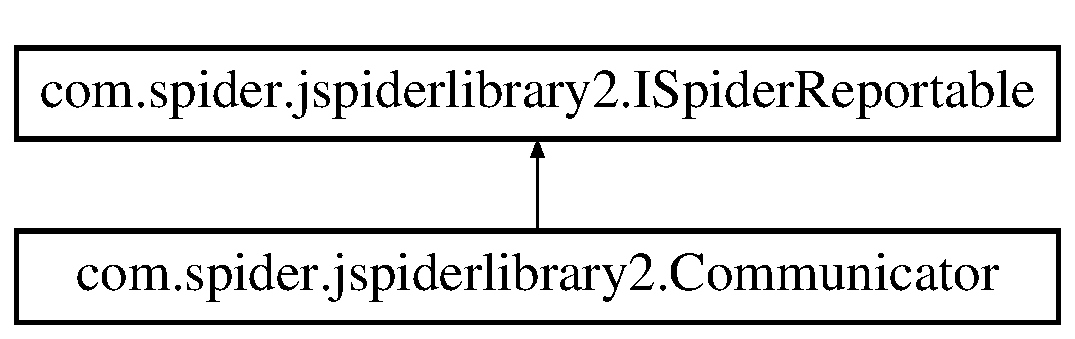
\includegraphics[height=2.000000cm]{classcom_1_1spider_1_1jspiderlibrary2_1_1_communicator}
\end{center}
\end{figure}
\subsection*{\-Public \-Member \-Functions}
\begin{DoxyCompactItemize}
\item 
void \hyperlink{classcom_1_1spider_1_1jspiderlibrary2_1_1_communicator_ab18b38c7ec6b8a8909267637649dd83a}{run} ()
\item 
void \hyperlink{classcom_1_1spider_1_1jspiderlibrary2_1_1_communicator_a41dd179b227fe3a5878f0b524d4ad1ad}{init\-Spider} ()
\item 
boolean \hyperlink{classcom_1_1spider_1_1jspiderlibrary2_1_1_communicator_a83fbf33e52836a135e944d0bde0cfd27}{spider\-Found\-U\-R\-L} (\-U\-R\-L \hyperlink{classcom_1_1spider_1_1jspiderlibrary2_1_1_communicator_ad0101fe504108054c599ff671b035ae7}{base}, \-U\-R\-L url)
\item 
void \hyperlink{classcom_1_1spider_1_1jspiderlibrary2_1_1_communicator_a18cc8b470895868f1d1fbf564c02e6f2}{spider\-Found\-U\-R\-L\-Error} (\-U\-R\-L url)
\end{DoxyCompactItemize}
\subsection*{\-Static \-Public \-Member \-Functions}
\begin{DoxyCompactItemize}
\item 
static \-Array\-List \hyperlink{classcom_1_1spider_1_1jspiderlibrary2_1_1_communicator_a4ff84ef1668376cdb43e76f0b376188c}{\-Search\-Engine\-Content\-To\-Ui} (\-Array\-List$<$ \-String $>$ list\-Of\-Links)
\end{DoxyCompactItemize}
\subsection*{\-Static \-Public \-Attributes}
\begin{DoxyCompactItemize}
\item 
static \-String \hyperlink{classcom_1_1spider_1_1jspiderlibrary2_1_1_communicator_a77d1d4556b66f56aad5fe9e1afda94d6}{text\-To\-Crawl}
\item 
static boolean \hyperlink{classcom_1_1spider_1_1jspiderlibrary2_1_1_communicator_aa0fb097a1e3dd28c5b3595965d0ebcd7}{crawl} = false
\item 
static boolean \hyperlink{classcom_1_1spider_1_1jspiderlibrary2_1_1_communicator_af0e22c130c8e3180b699325c5258bd83}{search} = false
\item 
static \-Hash\-Map \hyperlink{classcom_1_1spider_1_1jspiderlibrary2_1_1_communicator_a0c07a2143b8d612dd3a37f0ea948c458}{pages}
\item 
static int \hyperlink{classcom_1_1spider_1_1jspiderlibrary2_1_1_communicator_af85276b4b0e742776669cd6af974480c}{total\-Links}
\item 
static \-Array\-List \hyperlink{classcom_1_1spider_1_1jspiderlibrary2_1_1_communicator_ae6f31dbdb619cb67252f0c549ea8d81d}{linksprocessed} = new \-Array\-List()
\item 
static \-Array\-List \hyperlink{classcom_1_1spider_1_1jspiderlibrary2_1_1_communicator_ad9dc6cc7afc6f0203c1b5c723cd3cb06}{linkserror} = new \-Array\-List()
\end{DoxyCompactItemize}
\subsection*{\-Protected \-Member \-Functions}
\begin{DoxyCompactItemize}
\item 
boolean \hyperlink{classcom_1_1spider_1_1jspiderlibrary2_1_1_communicator_aa952bce8373401854579773a53fee26a}{check\-Link} (\-U\-R\-L url)
\end{DoxyCompactItemize}
\subsection*{\-Protected \-Attributes}
\begin{DoxyCompactItemize}
\item 
\hyperlink{classcom_1_1spider_1_1jspiderlibrary2_1_1_spider}{\-Spider} \hyperlink{classcom_1_1spider_1_1jspiderlibrary2_1_1_communicator_ad0dd6511cd30b7ad8edfd359a21c6cc3}{spider}
\item 
\-U\-R\-L \hyperlink{classcom_1_1spider_1_1jspiderlibrary2_1_1_communicator_ad0101fe504108054c599ff671b035ae7}{base}
\item 
int \hyperlink{classcom_1_1spider_1_1jspiderlibrary2_1_1_communicator_af90a1a8ad937a05d9b6058e669d28ca1}{bad\-Links\-Count} = 0
\item 
int \hyperlink{classcom_1_1spider_1_1jspiderlibrary2_1_1_communicator_a4d9dc7e33426c4efc3694340240bb568}{good\-Links\-Count} = 0
\end{DoxyCompactItemize}


\subsection{\-Detailed \-Description}
\begin{DoxyAuthor}{\-Author}
altamirano,peker,liberal 
\end{DoxyAuthor}


\-Definition at line 14 of file \-Communicator.\-java.



\subsection{\-Member \-Function \-Documentation}
\hypertarget{classcom_1_1spider_1_1jspiderlibrary2_1_1_communicator_aa952bce8373401854579773a53fee26a}{\index{com\-::spider\-::jspiderlibrary2\-::\-Communicator@{com\-::spider\-::jspiderlibrary2\-::\-Communicator}!check\-Link@{check\-Link}}
\index{check\-Link@{check\-Link}!com::spider::jspiderlibrary2::Communicator@{com\-::spider\-::jspiderlibrary2\-::\-Communicator}}
\subsubsection[{check\-Link}]{\setlength{\rightskip}{0pt plus 5cm}boolean {\bf com.\-spider.\-jspiderlibrary2.\-Communicator.\-check\-Link} (
\begin{DoxyParamCaption}
\item[{\-U\-R\-L}]{url}
\end{DoxyParamCaption}
)\hspace{0.3cm}{\ttfamily  \mbox{[}protected\mbox{]}}}}\label{classcom_1_1spider_1_1jspiderlibrary2_1_1_communicator_aa952bce8373401854579773a53fee26a}


\-Definition at line 94 of file \-Communicator.\-java.



\-Referenced by com.\-spider.\-jspiderlibrary2.\-Communicator.\-spider\-Found\-U\-R\-L().

\hypertarget{classcom_1_1spider_1_1jspiderlibrary2_1_1_communicator_a41dd179b227fe3a5878f0b524d4ad1ad}{\index{com\-::spider\-::jspiderlibrary2\-::\-Communicator@{com\-::spider\-::jspiderlibrary2\-::\-Communicator}!init\-Spider@{init\-Spider}}
\index{init\-Spider@{init\-Spider}!com::spider::jspiderlibrary2::Communicator@{com\-::spider\-::jspiderlibrary2\-::\-Communicator}}
\subsubsection[{init\-Spider}]{\setlength{\rightskip}{0pt plus 5cm}void {\bf com.\-spider.\-jspiderlibrary2.\-Communicator.\-init\-Spider} (
\begin{DoxyParamCaption}
{}
\end{DoxyParamCaption}
)}}\label{classcom_1_1spider_1_1jspiderlibrary2_1_1_communicator_a41dd179b227fe3a5878f0b524d4ad1ad}


\-Definition at line 54 of file \-Communicator.\-java.



\-References com.\-spider.\-jspiderlibrary2.\-Spider.\-add\-U\-R\-L(), com.\-spider.\-jspiderlibrary2.\-Communicator.\-base, com.\-spider.\-jspiderlibrary2.\-Spider.\-begin(), com.\-spider.\-jspiderlibrary2.\-Spider.\-clear(), com.\-spider.\-jspiderlibrary2.\-Communicator.\-spider, and com.\-spider.\-jspiderlibrary2.\-Communicator.\-text\-To\-Crawl.



\-Referenced by com.\-spider.\-jspiderlibrary2.\-Communicator.\-run().

\hypertarget{classcom_1_1spider_1_1jspiderlibrary2_1_1_communicator_ab18b38c7ec6b8a8909267637649dd83a}{\index{com\-::spider\-::jspiderlibrary2\-::\-Communicator@{com\-::spider\-::jspiderlibrary2\-::\-Communicator}!run@{run}}
\index{run@{run}!com::spider::jspiderlibrary2::Communicator@{com\-::spider\-::jspiderlibrary2\-::\-Communicator}}
\subsubsection[{run}]{\setlength{\rightskip}{0pt plus 5cm}void {\bf com.\-spider.\-jspiderlibrary2.\-Communicator.\-run} (
\begin{DoxyParamCaption}
{}
\end{DoxyParamCaption}
)}}\label{classcom_1_1spider_1_1jspiderlibrary2_1_1_communicator_ab18b38c7ec6b8a8909267637649dd83a}


\-Definition at line 34 of file \-Communicator.\-java.



\-References com.\-spider.\-jspiderlibrary2.\-Communicator.\-crawl, com.\-spider.\-jspiderlibrary2.\-Communicator.\-init\-Spider(), com.\-spider.\-jspiderlibrary2.\-Communicator.\-linkserror, com.\-spider.\-jspiderlibrary2.\-Communicator.\-linksprocessed, com.\-spider.\-jspiderlibrary2.\-Communicator.\-pages, com.\-spider.\-jspiderlibrary2.\-Communicator.\-spider, com.\-spider.\-jspiderlibrary2.\-Communicator.\-total\-Links, com.\-spider.\-jspiderlibrary2.\-Spider.\-workload\-Error, and com.\-spider.\-jspiderlibrary2.\-Spider.\-workload\-Processed.

\hypertarget{classcom_1_1spider_1_1jspiderlibrary2_1_1_communicator_a4ff84ef1668376cdb43e76f0b376188c}{\index{com\-::spider\-::jspiderlibrary2\-::\-Communicator@{com\-::spider\-::jspiderlibrary2\-::\-Communicator}!\-Search\-Engine\-Content\-To\-Ui@{\-Search\-Engine\-Content\-To\-Ui}}
\index{\-Search\-Engine\-Content\-To\-Ui@{\-Search\-Engine\-Content\-To\-Ui}!com::spider::jspiderlibrary2::Communicator@{com\-::spider\-::jspiderlibrary2\-::\-Communicator}}
\subsubsection[{\-Search\-Engine\-Content\-To\-Ui}]{\setlength{\rightskip}{0pt plus 5cm}static \-Array\-List {\bf com.\-spider.\-jspiderlibrary2.\-Communicator.\-Search\-Engine\-Content\-To\-Ui} (
\begin{DoxyParamCaption}
\item[{\-Array\-List$<$ \-String $>$}]{list\-Of\-Links}
\end{DoxyParamCaption}
)\hspace{0.3cm}{\ttfamily  \mbox{[}static\mbox{]}}}}\label{classcom_1_1spider_1_1jspiderlibrary2_1_1_communicator_a4ff84ef1668376cdb43e76f0b376188c}


\-Definition at line 113 of file \-Communicator.\-java.

\hypertarget{classcom_1_1spider_1_1jspiderlibrary2_1_1_communicator_a83fbf33e52836a135e944d0bde0cfd27}{\index{com\-::spider\-::jspiderlibrary2\-::\-Communicator@{com\-::spider\-::jspiderlibrary2\-::\-Communicator}!spider\-Found\-U\-R\-L@{spider\-Found\-U\-R\-L}}
\index{spider\-Found\-U\-R\-L@{spider\-Found\-U\-R\-L}!com::spider::jspiderlibrary2::Communicator@{com\-::spider\-::jspiderlibrary2\-::\-Communicator}}
\subsubsection[{spider\-Found\-U\-R\-L}]{\setlength{\rightskip}{0pt plus 5cm}boolean {\bf com.\-spider.\-jspiderlibrary2.\-Communicator.\-spider\-Found\-U\-R\-L} (
\begin{DoxyParamCaption}
\item[{\-U\-R\-L}]{base, }
\item[{\-U\-R\-L}]{url}
\end{DoxyParamCaption}
)}}\label{classcom_1_1spider_1_1jspiderlibrary2_1_1_communicator_a83fbf33e52836a135e944d0bde0cfd27}


\-Implements \hyperlink{interfacecom_1_1spider_1_1jspiderlibrary2_1_1_i_spider_reportable_a10fe4e486e6bd29efaa481e7532a84e3}{com.\-spider.\-jspiderlibrary2.\-I\-Spider\-Reportable}.



\-Definition at line 75 of file \-Communicator.\-java.



\-References com.\-spider.\-jspiderlibrary2.\-Communicator.\-bad\-Links\-Count, com.\-spider.\-jspiderlibrary2.\-Communicator.\-check\-Link(), and com.\-spider.\-jspiderlibrary2.\-Communicator.\-good\-Links\-Count.

\hypertarget{classcom_1_1spider_1_1jspiderlibrary2_1_1_communicator_a18cc8b470895868f1d1fbf564c02e6f2}{\index{com\-::spider\-::jspiderlibrary2\-::\-Communicator@{com\-::spider\-::jspiderlibrary2\-::\-Communicator}!spider\-Found\-U\-R\-L\-Error@{spider\-Found\-U\-R\-L\-Error}}
\index{spider\-Found\-U\-R\-L\-Error@{spider\-Found\-U\-R\-L\-Error}!com::spider::jspiderlibrary2::Communicator@{com\-::spider\-::jspiderlibrary2\-::\-Communicator}}
\subsubsection[{spider\-Found\-U\-R\-L\-Error}]{\setlength{\rightskip}{0pt plus 5cm}void {\bf com.\-spider.\-jspiderlibrary2.\-Communicator.\-spider\-Found\-U\-R\-L\-Error} (
\begin{DoxyParamCaption}
\item[{\-U\-R\-L}]{url}
\end{DoxyParamCaption}
)}}\label{classcom_1_1spider_1_1jspiderlibrary2_1_1_communicator_a18cc8b470895868f1d1fbf564c02e6f2}


\-Implements \hyperlink{interfacecom_1_1spider_1_1jspiderlibrary2_1_1_i_spider_reportable_a73e089019826aba4f610eaa4974e6ad8}{com.\-spider.\-jspiderlibrary2.\-I\-Spider\-Reportable}.



\-Definition at line 109 of file \-Communicator.\-java.



\-References com.\-spider.\-jspiderlibrary2.\-Communicator.\-bad\-Links\-Count.



\subsection{\-Member \-Data \-Documentation}
\hypertarget{classcom_1_1spider_1_1jspiderlibrary2_1_1_communicator_af90a1a8ad937a05d9b6058e669d28ca1}{\index{com\-::spider\-::jspiderlibrary2\-::\-Communicator@{com\-::spider\-::jspiderlibrary2\-::\-Communicator}!bad\-Links\-Count@{bad\-Links\-Count}}
\index{bad\-Links\-Count@{bad\-Links\-Count}!com::spider::jspiderlibrary2::Communicator@{com\-::spider\-::jspiderlibrary2\-::\-Communicator}}
\subsubsection[{bad\-Links\-Count}]{\setlength{\rightskip}{0pt plus 5cm}int {\bf com.\-spider.\-jspiderlibrary2.\-Communicator.\-bad\-Links\-Count} = 0\hspace{0.3cm}{\ttfamily  \mbox{[}protected\mbox{]}}}}\label{classcom_1_1spider_1_1jspiderlibrary2_1_1_communicator_af90a1a8ad937a05d9b6058e669d28ca1}


\-Definition at line 23 of file \-Communicator.\-java.



\-Referenced by com.\-spider.\-jspiderlibrary2.\-Communicator.\-spider\-Found\-U\-R\-L(), and com.\-spider.\-jspiderlibrary2.\-Communicator.\-spider\-Found\-U\-R\-L\-Error().

\hypertarget{classcom_1_1spider_1_1jspiderlibrary2_1_1_communicator_ad0101fe504108054c599ff671b035ae7}{\index{com\-::spider\-::jspiderlibrary2\-::\-Communicator@{com\-::spider\-::jspiderlibrary2\-::\-Communicator}!base@{base}}
\index{base@{base}!com::spider::jspiderlibrary2::Communicator@{com\-::spider\-::jspiderlibrary2\-::\-Communicator}}
\subsubsection[{base}]{\setlength{\rightskip}{0pt plus 5cm}\-U\-R\-L {\bf com.\-spider.\-jspiderlibrary2.\-Communicator.\-base}\hspace{0.3cm}{\ttfamily  \mbox{[}protected\mbox{]}}}}\label{classcom_1_1spider_1_1jspiderlibrary2_1_1_communicator_ad0101fe504108054c599ff671b035ae7}


\-Definition at line 22 of file \-Communicator.\-java.



\-Referenced by com.\-spider.\-jspiderlibrary2.\-Communicator.\-init\-Spider().

\hypertarget{classcom_1_1spider_1_1jspiderlibrary2_1_1_communicator_aa0fb097a1e3dd28c5b3595965d0ebcd7}{\index{com\-::spider\-::jspiderlibrary2\-::\-Communicator@{com\-::spider\-::jspiderlibrary2\-::\-Communicator}!crawl@{crawl}}
\index{crawl@{crawl}!com::spider::jspiderlibrary2::Communicator@{com\-::spider\-::jspiderlibrary2\-::\-Communicator}}
\subsubsection[{crawl}]{\setlength{\rightskip}{0pt plus 5cm}boolean {\bf com.\-spider.\-jspiderlibrary2.\-Communicator.\-crawl} = false\hspace{0.3cm}{\ttfamily  \mbox{[}static\mbox{]}}}}\label{classcom_1_1spider_1_1jspiderlibrary2_1_1_communicator_aa0fb097a1e3dd28c5b3595965d0ebcd7}


\-Definition at line 19 of file \-Communicator.\-java.



\-Referenced by com.\-spider.\-jspiderlibrary2.\-Communicator.\-run().

\hypertarget{classcom_1_1spider_1_1jspiderlibrary2_1_1_communicator_a4d9dc7e33426c4efc3694340240bb568}{\index{com\-::spider\-::jspiderlibrary2\-::\-Communicator@{com\-::spider\-::jspiderlibrary2\-::\-Communicator}!good\-Links\-Count@{good\-Links\-Count}}
\index{good\-Links\-Count@{good\-Links\-Count}!com::spider::jspiderlibrary2::Communicator@{com\-::spider\-::jspiderlibrary2\-::\-Communicator}}
\subsubsection[{good\-Links\-Count}]{\setlength{\rightskip}{0pt plus 5cm}int {\bf com.\-spider.\-jspiderlibrary2.\-Communicator.\-good\-Links\-Count} = 0\hspace{0.3cm}{\ttfamily  \mbox{[}protected\mbox{]}}}}\label{classcom_1_1spider_1_1jspiderlibrary2_1_1_communicator_a4d9dc7e33426c4efc3694340240bb568}


\-Definition at line 24 of file \-Communicator.\-java.



\-Referenced by com.\-spider.\-jspiderlibrary2.\-Communicator.\-spider\-Found\-U\-R\-L().

\hypertarget{classcom_1_1spider_1_1jspiderlibrary2_1_1_communicator_ad9dc6cc7afc6f0203c1b5c723cd3cb06}{\index{com\-::spider\-::jspiderlibrary2\-::\-Communicator@{com\-::spider\-::jspiderlibrary2\-::\-Communicator}!linkserror@{linkserror}}
\index{linkserror@{linkserror}!com::spider::jspiderlibrary2::Communicator@{com\-::spider\-::jspiderlibrary2\-::\-Communicator}}
\subsubsection[{linkserror}]{\setlength{\rightskip}{0pt plus 5cm}\-Array\-List {\bf com.\-spider.\-jspiderlibrary2.\-Communicator.\-linkserror} = new \-Array\-List()\hspace{0.3cm}{\ttfamily  \mbox{[}static\mbox{]}}}}\label{classcom_1_1spider_1_1jspiderlibrary2_1_1_communicator_ad9dc6cc7afc6f0203c1b5c723cd3cb06}


\-Definition at line 28 of file \-Communicator.\-java.



\-Referenced by com.\-spider.\-jspiderlibrary2.\-Communicator.\-run().

\hypertarget{classcom_1_1spider_1_1jspiderlibrary2_1_1_communicator_ae6f31dbdb619cb67252f0c549ea8d81d}{\index{com\-::spider\-::jspiderlibrary2\-::\-Communicator@{com\-::spider\-::jspiderlibrary2\-::\-Communicator}!linksprocessed@{linksprocessed}}
\index{linksprocessed@{linksprocessed}!com::spider::jspiderlibrary2::Communicator@{com\-::spider\-::jspiderlibrary2\-::\-Communicator}}
\subsubsection[{linksprocessed}]{\setlength{\rightskip}{0pt plus 5cm}\-Array\-List {\bf com.\-spider.\-jspiderlibrary2.\-Communicator.\-linksprocessed} = new \-Array\-List()\hspace{0.3cm}{\ttfamily  \mbox{[}static\mbox{]}}}}\label{classcom_1_1spider_1_1jspiderlibrary2_1_1_communicator_ae6f31dbdb619cb67252f0c549ea8d81d}


\-Definition at line 27 of file \-Communicator.\-java.



\-Referenced by com.\-spider.\-jspiderlibrary2.\-Communicator.\-run().

\hypertarget{classcom_1_1spider_1_1jspiderlibrary2_1_1_communicator_a0c07a2143b8d612dd3a37f0ea948c458}{\index{com\-::spider\-::jspiderlibrary2\-::\-Communicator@{com\-::spider\-::jspiderlibrary2\-::\-Communicator}!pages@{pages}}
\index{pages@{pages}!com::spider::jspiderlibrary2::Communicator@{com\-::spider\-::jspiderlibrary2\-::\-Communicator}}
\subsubsection[{pages}]{\setlength{\rightskip}{0pt plus 5cm}\-Hash\-Map {\bf com.\-spider.\-jspiderlibrary2.\-Communicator.\-pages}\hspace{0.3cm}{\ttfamily  \mbox{[}static\mbox{]}}}}\label{classcom_1_1spider_1_1jspiderlibrary2_1_1_communicator_a0c07a2143b8d612dd3a37f0ea948c458}


\-Definition at line 25 of file \-Communicator.\-java.



\-Referenced by com.\-spider.\-jspiderlibrary2.\-Communicator.\-run().

\hypertarget{classcom_1_1spider_1_1jspiderlibrary2_1_1_communicator_af0e22c130c8e3180b699325c5258bd83}{\index{com\-::spider\-::jspiderlibrary2\-::\-Communicator@{com\-::spider\-::jspiderlibrary2\-::\-Communicator}!search@{search}}
\index{search@{search}!com::spider::jspiderlibrary2::Communicator@{com\-::spider\-::jspiderlibrary2\-::\-Communicator}}
\subsubsection[{search}]{\setlength{\rightskip}{0pt plus 5cm}boolean {\bf com.\-spider.\-jspiderlibrary2.\-Communicator.\-search} = false\hspace{0.3cm}{\ttfamily  \mbox{[}static\mbox{]}}}}\label{classcom_1_1spider_1_1jspiderlibrary2_1_1_communicator_af0e22c130c8e3180b699325c5258bd83}


\-Definition at line 20 of file \-Communicator.\-java.

\hypertarget{classcom_1_1spider_1_1jspiderlibrary2_1_1_communicator_ad0dd6511cd30b7ad8edfd359a21c6cc3}{\index{com\-::spider\-::jspiderlibrary2\-::\-Communicator@{com\-::spider\-::jspiderlibrary2\-::\-Communicator}!spider@{spider}}
\index{spider@{spider}!com::spider::jspiderlibrary2::Communicator@{com\-::spider\-::jspiderlibrary2\-::\-Communicator}}
\subsubsection[{spider}]{\setlength{\rightskip}{0pt plus 5cm}{\bf \-Spider} {\bf com.\-spider.\-jspiderlibrary2.\-Communicator.\-spider}\hspace{0.3cm}{\ttfamily  \mbox{[}protected\mbox{]}}}}\label{classcom_1_1spider_1_1jspiderlibrary2_1_1_communicator_ad0dd6511cd30b7ad8edfd359a21c6cc3}


\-Definition at line 21 of file \-Communicator.\-java.



\-Referenced by com.\-spider.\-jspiderlibrary2.\-Communicator.\-init\-Spider(), and com.\-spider.\-jspiderlibrary2.\-Communicator.\-run().

\hypertarget{classcom_1_1spider_1_1jspiderlibrary2_1_1_communicator_a77d1d4556b66f56aad5fe9e1afda94d6}{\index{com\-::spider\-::jspiderlibrary2\-::\-Communicator@{com\-::spider\-::jspiderlibrary2\-::\-Communicator}!text\-To\-Crawl@{text\-To\-Crawl}}
\index{text\-To\-Crawl@{text\-To\-Crawl}!com::spider::jspiderlibrary2::Communicator@{com\-::spider\-::jspiderlibrary2\-::\-Communicator}}
\subsubsection[{text\-To\-Crawl}]{\setlength{\rightskip}{0pt plus 5cm}\-String {\bf com.\-spider.\-jspiderlibrary2.\-Communicator.\-text\-To\-Crawl}\hspace{0.3cm}{\ttfamily  \mbox{[}static\mbox{]}}}}\label{classcom_1_1spider_1_1jspiderlibrary2_1_1_communicator_a77d1d4556b66f56aad5fe9e1afda94d6}


\-Definition at line 17 of file \-Communicator.\-java.



\-Referenced by com.\-spider.\-jspiderlibrary2.\-Communicator.\-init\-Spider().

\hypertarget{classcom_1_1spider_1_1jspiderlibrary2_1_1_communicator_af85276b4b0e742776669cd6af974480c}{\index{com\-::spider\-::jspiderlibrary2\-::\-Communicator@{com\-::spider\-::jspiderlibrary2\-::\-Communicator}!total\-Links@{total\-Links}}
\index{total\-Links@{total\-Links}!com::spider::jspiderlibrary2::Communicator@{com\-::spider\-::jspiderlibrary2\-::\-Communicator}}
\subsubsection[{total\-Links}]{\setlength{\rightskip}{0pt plus 5cm}int {\bf com.\-spider.\-jspiderlibrary2.\-Communicator.\-total\-Links}\hspace{0.3cm}{\ttfamily  \mbox{[}static\mbox{]}}}}\label{classcom_1_1spider_1_1jspiderlibrary2_1_1_communicator_af85276b4b0e742776669cd6af974480c}


\-Definition at line 26 of file \-Communicator.\-java.



\-Referenced by com.\-spider.\-jspiderlibrary2.\-Spider.\-process\-U\-R\-L(), and com.\-spider.\-jspiderlibrary2.\-Communicator.\-run().



\-The documentation for this class was generated from the following file\-:\begin{DoxyCompactItemize}
\item 
src/main/java/com/spider/jspiderlibrary2/\hyperlink{_communicator_8java}{\-Communicator.\-java}\end{DoxyCompactItemize}

\hypertarget{classcom_1_1spider_1_1jspiderlibrary2_1_1_h_t_m_l_parse}{\section{com.\-spider.\-jspiderlibrary2.\-H\-T\-M\-L\-Parse \-Class \-Reference}
\label{classcom_1_1spider_1_1jspiderlibrary2_1_1_h_t_m_l_parse}\index{com.\-spider.\-jspiderlibrary2.\-H\-T\-M\-L\-Parse@{com.\-spider.\-jspiderlibrary2.\-H\-T\-M\-L\-Parse}}
}


\-Inherits \-H\-T\-M\-L\-Editor\-Kit.

\subsection*{\-Public \-Member \-Functions}
\begin{DoxyCompactItemize}
\item 
\-H\-T\-M\-L\-Editor\-Kit.\-Parser \hyperlink{classcom_1_1spider_1_1jspiderlibrary2_1_1_h_t_m_l_parse_a490841fe99ac950af2fe545785edadae}{get\-Parser} ()
\end{DoxyCompactItemize}


\subsection{\-Detailed \-Description}
\begin{DoxyAuthor}{\-Author}
altamirano,peker,liberal 
\end{DoxyAuthor}


\-Definition at line 11 of file \-H\-T\-M\-L\-Parse.\-java.



\subsection{\-Member \-Function \-Documentation}
\hypertarget{classcom_1_1spider_1_1jspiderlibrary2_1_1_h_t_m_l_parse_a490841fe99ac950af2fe545785edadae}{\index{com\-::spider\-::jspiderlibrary2\-::\-H\-T\-M\-L\-Parse@{com\-::spider\-::jspiderlibrary2\-::\-H\-T\-M\-L\-Parse}!get\-Parser@{get\-Parser}}
\index{get\-Parser@{get\-Parser}!com::spider::jspiderlibrary2::HTMLParse@{com\-::spider\-::jspiderlibrary2\-::\-H\-T\-M\-L\-Parse}}
\subsubsection[{get\-Parser}]{\setlength{\rightskip}{0pt plus 5cm}\-H\-T\-M\-L\-Editor\-Kit.\-Parser {\bf com.\-spider.\-jspiderlibrary2.\-H\-T\-M\-L\-Parse.\-get\-Parser} (
\begin{DoxyParamCaption}
{}
\end{DoxyParamCaption}
)}}\label{classcom_1_1spider_1_1jspiderlibrary2_1_1_h_t_m_l_parse_a490841fe99ac950af2fe545785edadae}


\-Definition at line 15 of file \-H\-T\-M\-L\-Parse.\-java.



\-Referenced by com.\-spider.\-jspiderlibrary2.\-Spider.\-process\-U\-R\-L().



\-The documentation for this class was generated from the following file\-:\begin{DoxyCompactItemize}
\item 
src/main/java/com/spider/jspiderlibrary2/\hyperlink{_h_t_m_l_parse_8java}{\-H\-T\-M\-L\-Parse.\-java}\end{DoxyCompactItemize}

\hypertarget{interfacecom_1_1spider_1_1jspiderlibrary2_1_1_i_spider_reportable}{\section{com.\-spider.\-jspiderlibrary2.\-I\-Spider\-Reportable \-Interface \-Reference}
\label{interfacecom_1_1spider_1_1jspiderlibrary2_1_1_i_spider_reportable}\index{com.\-spider.\-jspiderlibrary2.\-I\-Spider\-Reportable@{com.\-spider.\-jspiderlibrary2.\-I\-Spider\-Reportable}}
}
\-Inheritance diagram for com.\-spider.\-jspiderlibrary2.\-I\-Spider\-Reportable\-:\begin{figure}[H]
\begin{center}
\leavevmode
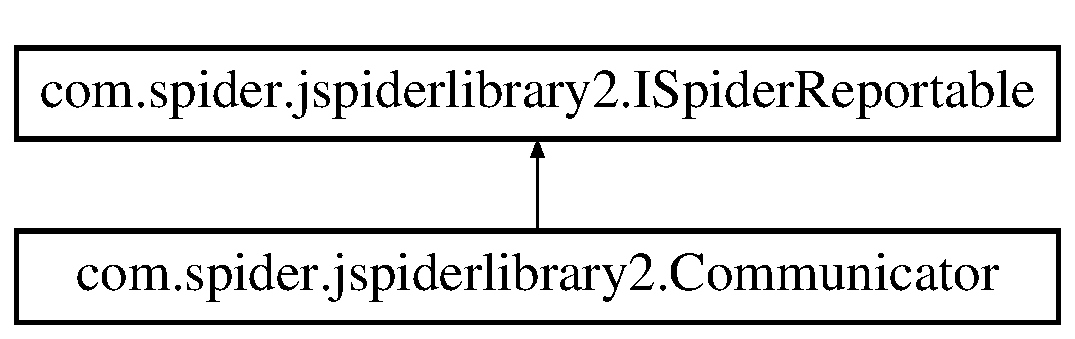
\includegraphics[height=2.000000cm]{interfacecom_1_1spider_1_1jspiderlibrary2_1_1_i_spider_reportable}
\end{center}
\end{figure}
\subsection*{\-Public \-Member \-Functions}
\begin{DoxyCompactItemize}
\item 
boolean \hyperlink{interfacecom_1_1spider_1_1jspiderlibrary2_1_1_i_spider_reportable_a10fe4e486e6bd29efaa481e7532a84e3}{spider\-Found\-U\-R\-L} (\-U\-R\-L base, \-U\-R\-L url)
\item 
void \hyperlink{interfacecom_1_1spider_1_1jspiderlibrary2_1_1_i_spider_reportable_a73e089019826aba4f610eaa4974e6ad8}{spider\-Found\-U\-R\-L\-Error} (\-U\-R\-L url)
\end{DoxyCompactItemize}


\subsection{\-Detailed \-Description}
\begin{DoxyAuthor}{\-Author}
altamirano,peker,liberal 
\end{DoxyAuthor}


\-Definition at line 13 of file \-I\-Spider\-Reportable.\-java.



\subsection{\-Member \-Function \-Documentation}
\hypertarget{interfacecom_1_1spider_1_1jspiderlibrary2_1_1_i_spider_reportable_a10fe4e486e6bd29efaa481e7532a84e3}{\index{com\-::spider\-::jspiderlibrary2\-::\-I\-Spider\-Reportable@{com\-::spider\-::jspiderlibrary2\-::\-I\-Spider\-Reportable}!spider\-Found\-U\-R\-L@{spider\-Found\-U\-R\-L}}
\index{spider\-Found\-U\-R\-L@{spider\-Found\-U\-R\-L}!com::spider::jspiderlibrary2::ISpiderReportable@{com\-::spider\-::jspiderlibrary2\-::\-I\-Spider\-Reportable}}
\subsubsection[{spider\-Found\-U\-R\-L}]{\setlength{\rightskip}{0pt plus 5cm}boolean {\bf com.\-spider.\-jspiderlibrary2.\-I\-Spider\-Reportable.\-spider\-Found\-U\-R\-L} (
\begin{DoxyParamCaption}
\item[{\-U\-R\-L}]{base, }
\item[{\-U\-R\-L}]{url}
\end{DoxyParamCaption}
)}}\label{interfacecom_1_1spider_1_1jspiderlibrary2_1_1_i_spider_reportable_a10fe4e486e6bd29efaa481e7532a84e3}


\-Implemented in \hyperlink{classcom_1_1spider_1_1jspiderlibrary2_1_1_communicator_a83fbf33e52836a135e944d0bde0cfd27}{com.\-spider.\-jspiderlibrary2.\-Communicator}.



\-Referenced by com.\-spider.\-jspiderlibrary2.\-Spider.\-Parser.\-handle\-Link().

\hypertarget{interfacecom_1_1spider_1_1jspiderlibrary2_1_1_i_spider_reportable_a73e089019826aba4f610eaa4974e6ad8}{\index{com\-::spider\-::jspiderlibrary2\-::\-I\-Spider\-Reportable@{com\-::spider\-::jspiderlibrary2\-::\-I\-Spider\-Reportable}!spider\-Found\-U\-R\-L\-Error@{spider\-Found\-U\-R\-L\-Error}}
\index{spider\-Found\-U\-R\-L\-Error@{spider\-Found\-U\-R\-L\-Error}!com::spider::jspiderlibrary2::ISpiderReportable@{com\-::spider\-::jspiderlibrary2\-::\-I\-Spider\-Reportable}}
\subsubsection[{spider\-Found\-U\-R\-L\-Error}]{\setlength{\rightskip}{0pt plus 5cm}void {\bf com.\-spider.\-jspiderlibrary2.\-I\-Spider\-Reportable.\-spider\-Found\-U\-R\-L\-Error} (
\begin{DoxyParamCaption}
\item[{\-U\-R\-L}]{url}
\end{DoxyParamCaption}
)}}\label{interfacecom_1_1spider_1_1jspiderlibrary2_1_1_i_spider_reportable_a73e089019826aba4f610eaa4974e6ad8}


\-Implemented in \hyperlink{classcom_1_1spider_1_1jspiderlibrary2_1_1_communicator_a18cc8b470895868f1d1fbf564c02e6f2}{com.\-spider.\-jspiderlibrary2.\-Communicator}.



\-Referenced by com.\-spider.\-jspiderlibrary2.\-Spider.\-process\-U\-R\-L().



\-The documentation for this interface was generated from the following file\-:\begin{DoxyCompactItemize}
\item 
src/main/java/com/spider/jspiderlibrary2/\hyperlink{_i_spider_reportable_8java}{\-I\-Spider\-Reportable.\-java}\end{DoxyCompactItemize}

\hypertarget{classcom_1_1spider_1_1jspiderlibrary2_1_1_spider_1_1_parser}{\section{com.\-spider.\-jspiderlibrary2.\-Spider.\-Parser \-Class \-Reference}
\label{classcom_1_1spider_1_1jspiderlibrary2_1_1_spider_1_1_parser}\index{com.\-spider.\-jspiderlibrary2.\-Spider.\-Parser@{com.\-spider.\-jspiderlibrary2.\-Spider.\-Parser}}
}
\subsection*{\-Public \-Member \-Functions}
\begin{DoxyCompactItemize}
\item 
\hyperlink{classcom_1_1spider_1_1jspiderlibrary2_1_1_spider_1_1_parser_a72ae3a543c9a4538a39e552b7118bd6d}{\-Parser} (\-U\-R\-L \hyperlink{classcom_1_1spider_1_1jspiderlibrary2_1_1_spider_1_1_parser_aaac5fcd0aa0bdd67e4c6842d2657231d}{base})
\item 
void \hyperlink{classcom_1_1spider_1_1jspiderlibrary2_1_1_spider_1_1_parser_a04eb14f6a2105866c962a0b1bdc9c568}{tag\-Handler} (\-H\-T\-M\-L.\-Tag tag)
\item 
void \hyperlink{classcom_1_1spider_1_1jspiderlibrary2_1_1_spider_1_1_parser_ae14a442ac7232170e7db1e8f872d6f8a}{handle\-Simple\-Tag} (\-H\-T\-M\-L.\-Tag tag, \-Mutable\-Attribute\-Set atribute\-Set, int pos)
\item 
void \hyperlink{classcom_1_1spider_1_1jspiderlibrary2_1_1_spider_1_1_parser_a1a351dca2ed508a436546687e782d329}{handle\-Start\-Tag} (\-H\-T\-M\-L.\-Tag t, \-Mutable\-Attribute\-Set a, int pos)
\item 
void \hyperlink{classcom_1_1spider_1_1jspiderlibrary2_1_1_spider_1_1_parser_a293631e270d69e91a29de14c980bc9c8}{handle\-Text} (char\mbox{[}$\,$\mbox{]} data, int pos)
\end{DoxyCompactItemize}
\subsection*{\-Protected \-Member \-Functions}
\begin{DoxyCompactItemize}
\item 
void \hyperlink{classcom_1_1spider_1_1jspiderlibrary2_1_1_spider_1_1_parser_aa7bd808ea40da16b1e666113db1b1616}{handle\-Link} (\-U\-R\-L \hyperlink{classcom_1_1spider_1_1jspiderlibrary2_1_1_spider_1_1_parser_aaac5fcd0aa0bdd67e4c6842d2657231d}{base}, \-String str)
\end{DoxyCompactItemize}
\subsection*{\-Protected \-Attributes}
\begin{DoxyCompactItemize}
\item 
\-U\-R\-L \hyperlink{classcom_1_1spider_1_1jspiderlibrary2_1_1_spider_1_1_parser_aaac5fcd0aa0bdd67e4c6842d2657231d}{base}
\end{DoxyCompactItemize}


\subsection{\-Detailed \-Description}
\-Creo un parser de \-H\-T\-M\-L en funcion de la clase \-H\-T\-M\-L editor empleada para parsear y detectar los links 

\-Definition at line 253 of file \-Spider.\-java.



\subsection{\-Constructor \& \-Destructor \-Documentation}
\hypertarget{classcom_1_1spider_1_1jspiderlibrary2_1_1_spider_1_1_parser_a72ae3a543c9a4538a39e552b7118bd6d}{\index{com\-::spider\-::jspiderlibrary2\-::\-Spider\-::\-Parser@{com\-::spider\-::jspiderlibrary2\-::\-Spider\-::\-Parser}!\-Parser@{\-Parser}}
\index{\-Parser@{\-Parser}!com::spider::jspiderlibrary2::Spider::Parser@{com\-::spider\-::jspiderlibrary2\-::\-Spider\-::\-Parser}}
\subsubsection[{\-Parser}]{\setlength{\rightskip}{0pt plus 5cm}{\bf com.\-spider.\-jspiderlibrary2.\-Spider.\-Parser.\-Parser} (
\begin{DoxyParamCaption}
\item[{\-U\-R\-L}]{base}
\end{DoxyParamCaption}
)}}\label{classcom_1_1spider_1_1jspiderlibrary2_1_1_spider_1_1_parser_a72ae3a543c9a4538a39e552b7118bd6d}


\-Definition at line 261 of file \-Spider.\-java.



\-References com.\-spider.\-jspiderlibrary2.\-Spider.\-Parser.\-base.



\subsection{\-Member \-Function \-Documentation}
\hypertarget{classcom_1_1spider_1_1jspiderlibrary2_1_1_spider_1_1_parser_aa7bd808ea40da16b1e666113db1b1616}{\index{com\-::spider\-::jspiderlibrary2\-::\-Spider\-::\-Parser@{com\-::spider\-::jspiderlibrary2\-::\-Spider\-::\-Parser}!handle\-Link@{handle\-Link}}
\index{handle\-Link@{handle\-Link}!com::spider::jspiderlibrary2::Spider::Parser@{com\-::spider\-::jspiderlibrary2\-::\-Spider\-::\-Parser}}
\subsubsection[{handle\-Link}]{\setlength{\rightskip}{0pt plus 5cm}void {\bf com.\-spider.\-jspiderlibrary2.\-Spider.\-Parser.\-handle\-Link} (
\begin{DoxyParamCaption}
\item[{\-U\-R\-L}]{base, }
\item[{\-String}]{str}
\end{DoxyParamCaption}
)\hspace{0.3cm}{\ttfamily  \mbox{[}protected\mbox{]}}}}\label{classcom_1_1spider_1_1jspiderlibrary2_1_1_spider_1_1_parser_aa7bd808ea40da16b1e666113db1b1616}

\begin{DoxyParams}{\-Parameters}
{\em base} & \\
\hline
{\em str} & \\
\hline
\end{DoxyParams}


\-Definition at line 397 of file \-Spider.\-java.



\-References com.\-spider.\-jspiderlibrary2.\-Spider.\-add\-U\-R\-L(), com.\-spider.\-jspiderlibrary2.\-Spider.\-log(), com.\-spider.\-jspiderlibrary2.\-Spider.\-report, and com.\-spider.\-jspiderlibrary2.\-I\-Spider\-Reportable.\-spider\-Found\-U\-R\-L().



\-Referenced by com.\-spider.\-jspiderlibrary2.\-Spider.\-Parser.\-handle\-Simple\-Tag().

\hypertarget{classcom_1_1spider_1_1jspiderlibrary2_1_1_spider_1_1_parser_ae14a442ac7232170e7db1e8f872d6f8a}{\index{com\-::spider\-::jspiderlibrary2\-::\-Spider\-::\-Parser@{com\-::spider\-::jspiderlibrary2\-::\-Spider\-::\-Parser}!handle\-Simple\-Tag@{handle\-Simple\-Tag}}
\index{handle\-Simple\-Tag@{handle\-Simple\-Tag}!com::spider::jspiderlibrary2::Spider::Parser@{com\-::spider\-::jspiderlibrary2\-::\-Spider\-::\-Parser}}
\subsubsection[{handle\-Simple\-Tag}]{\setlength{\rightskip}{0pt plus 5cm}void {\bf com.\-spider.\-jspiderlibrary2.\-Spider.\-Parser.\-handle\-Simple\-Tag} (
\begin{DoxyParamCaption}
\item[{\-H\-T\-M\-L.\-Tag}]{tag, }
\item[{\-Mutable\-Attribute\-Set}]{atribute\-Set, }
\item[{int}]{pos}
\end{DoxyParamCaption}
)}}\label{classcom_1_1spider_1_1jspiderlibrary2_1_1_spider_1_1_parser_ae14a442ac7232170e7db1e8f872d6f8a}


\-Definition at line 295 of file \-Spider.\-java.



\-References com.\-spider.\-jspiderlibrary2.\-Spider.\-Parser.\-base, com.\-spider.\-jspiderlibrary2.\-Spider.\-Parser.\-handle\-Link(), and com.\-spider.\-jspiderlibrary2.\-Spider.\-Parser.\-tag\-Handler().



\-Referenced by com.\-spider.\-jspiderlibrary2.\-Spider.\-Parser.\-handle\-Start\-Tag().

\hypertarget{classcom_1_1spider_1_1jspiderlibrary2_1_1_spider_1_1_parser_a1a351dca2ed508a436546687e782d329}{\index{com\-::spider\-::jspiderlibrary2\-::\-Spider\-::\-Parser@{com\-::spider\-::jspiderlibrary2\-::\-Spider\-::\-Parser}!handle\-Start\-Tag@{handle\-Start\-Tag}}
\index{handle\-Start\-Tag@{handle\-Start\-Tag}!com::spider::jspiderlibrary2::Spider::Parser@{com\-::spider\-::jspiderlibrary2\-::\-Spider\-::\-Parser}}
\subsubsection[{handle\-Start\-Tag}]{\setlength{\rightskip}{0pt plus 5cm}void {\bf com.\-spider.\-jspiderlibrary2.\-Spider.\-Parser.\-handle\-Start\-Tag} (
\begin{DoxyParamCaption}
\item[{\-H\-T\-M\-L.\-Tag}]{t, }
\item[{\-Mutable\-Attribute\-Set}]{a, }
\item[{int}]{pos}
\end{DoxyParamCaption}
)}}\label{classcom_1_1spider_1_1jspiderlibrary2_1_1_spider_1_1_parser_a1a351dca2ed508a436546687e782d329}


\-Definition at line 357 of file \-Spider.\-java.



\-References com.\-spider.\-jspiderlibrary2.\-Spider.\-Parser.\-handle\-Simple\-Tag().

\hypertarget{classcom_1_1spider_1_1jspiderlibrary2_1_1_spider_1_1_parser_a293631e270d69e91a29de14c980bc9c8}{\index{com\-::spider\-::jspiderlibrary2\-::\-Spider\-::\-Parser@{com\-::spider\-::jspiderlibrary2\-::\-Spider\-::\-Parser}!handle\-Text@{handle\-Text}}
\index{handle\-Text@{handle\-Text}!com::spider::jspiderlibrary2::Spider::Parser@{com\-::spider\-::jspiderlibrary2\-::\-Spider\-::\-Parser}}
\subsubsection[{handle\-Text}]{\setlength{\rightskip}{0pt plus 5cm}void {\bf com.\-spider.\-jspiderlibrary2.\-Spider.\-Parser.\-handle\-Text} (
\begin{DoxyParamCaption}
\item[{char\mbox{[}$\,$\mbox{]}}]{data, }
\item[{int}]{pos}
\end{DoxyParamCaption}
)}}\label{classcom_1_1spider_1_1jspiderlibrary2_1_1_spider_1_1_parser_a293631e270d69e91a29de14c980bc9c8}

\begin{DoxyParams}{\-Parameters}
{\em data} & gots the tag text \\
\hline
{\em pos} & \\
\hline
\end{DoxyParams}


\-Definition at line 368 of file \-Spider.\-java.

\hypertarget{classcom_1_1spider_1_1jspiderlibrary2_1_1_spider_1_1_parser_a04eb14f6a2105866c962a0b1bdc9c568}{\index{com\-::spider\-::jspiderlibrary2\-::\-Spider\-::\-Parser@{com\-::spider\-::jspiderlibrary2\-::\-Spider\-::\-Parser}!tag\-Handler@{tag\-Handler}}
\index{tag\-Handler@{tag\-Handler}!com::spider::jspiderlibrary2::Spider::Parser@{com\-::spider\-::jspiderlibrary2\-::\-Spider\-::\-Parser}}
\subsubsection[{tag\-Handler}]{\setlength{\rightskip}{0pt plus 5cm}void {\bf com.\-spider.\-jspiderlibrary2.\-Spider.\-Parser.\-tag\-Handler} (
\begin{DoxyParamCaption}
\item[{\-H\-T\-M\-L.\-Tag}]{tag}
\end{DoxyParamCaption}
)}}\label{classcom_1_1spider_1_1jspiderlibrary2_1_1_spider_1_1_parser_a04eb14f6a2105866c962a0b1bdc9c568}
\-Verifico si existen tags indeseados, es decir tags que no deben tener texto comparo el tag actual con el tag indeseado, con eso seteo el flag para notificarle al handle\-Text que el tag \-N\-O debe ser procesado 
\begin{DoxyParams}{\-Parameters}
{\em tag} & a \-H\-T\-M\-L.\-Tag \\
\hline
\end{DoxyParams}


\-Definition at line 272 of file \-Spider.\-java.



\-Referenced by com.\-spider.\-jspiderlibrary2.\-Spider.\-Parser.\-handle\-Simple\-Tag().



\subsection{\-Member \-Data \-Documentation}
\hypertarget{classcom_1_1spider_1_1jspiderlibrary2_1_1_spider_1_1_parser_aaac5fcd0aa0bdd67e4c6842d2657231d}{\index{com\-::spider\-::jspiderlibrary2\-::\-Spider\-::\-Parser@{com\-::spider\-::jspiderlibrary2\-::\-Spider\-::\-Parser}!base@{base}}
\index{base@{base}!com::spider::jspiderlibrary2::Spider::Parser@{com\-::spider\-::jspiderlibrary2\-::\-Spider\-::\-Parser}}
\subsubsection[{base}]{\setlength{\rightskip}{0pt plus 5cm}\-U\-R\-L {\bf com.\-spider.\-jspiderlibrary2.\-Spider.\-Parser.\-base}\hspace{0.3cm}{\ttfamily  \mbox{[}protected\mbox{]}}}}\label{classcom_1_1spider_1_1jspiderlibrary2_1_1_spider_1_1_parser_aaac5fcd0aa0bdd67e4c6842d2657231d}


\-Definition at line 257 of file \-Spider.\-java.



\-Referenced by com.\-spider.\-jspiderlibrary2.\-Spider.\-Parser.\-handle\-Simple\-Tag(), and com.\-spider.\-jspiderlibrary2.\-Spider.\-Parser.\-Parser().



\-The documentation for this class was generated from the following file\-:\begin{DoxyCompactItemize}
\item 
src/main/java/com/spider/jspiderlibrary2/\hyperlink{_spider_8java}{\-Spider.\-java}\end{DoxyCompactItemize}

\hypertarget{classcom_1_1spider_1_1jspiderlibrary2_1_1_robots_parser}{\section{com.\-spider.\-jspiderlibrary2.\-Robots\-Parser \-Class \-Reference}
\label{classcom_1_1spider_1_1jspiderlibrary2_1_1_robots_parser}\index{com.\-spider.\-jspiderlibrary2.\-Robots\-Parser@{com.\-spider.\-jspiderlibrary2.\-Robots\-Parser}}
}
\subsection*{\-Static \-Public \-Member \-Functions}
\begin{DoxyCompactItemize}
\item 
static boolean \hyperlink{classcom_1_1spider_1_1jspiderlibrary2_1_1_robots_parser_a763eb021063080b7cbfc3a0477b89b38}{robot\-Safe} (\-U\-R\-L url)
\end{DoxyCompactItemize}
\subsection*{\-Static \-Public \-Attributes}
\begin{DoxyCompactItemize}
\item 
static final \-String \hyperlink{classcom_1_1spider_1_1jspiderlibrary2_1_1_robots_parser_a0455347c6ace914cb64885d5cb4e051b}{\-S\-E\-A\-R\-C\-H} = \char`\"{}\-Search\char`\"{}
\item 
static final \-String \hyperlink{classcom_1_1spider_1_1jspiderlibrary2_1_1_robots_parser_aff7a48bec0d0fa25e624afcc60144f32}{\-S\-T\-O\-P} = \char`\"{}\-Stop\char`\"{}
\item 
static final \-String \hyperlink{classcom_1_1spider_1_1jspiderlibrary2_1_1_robots_parser_a0d4b2f94e6784a8bff783928ef5d5a78}{\-D\-I\-S\-A\-L\-L\-O\-W} = \char`\"{}\-Disallow\-:\char`\"{}
\item 
static final int \hyperlink{classcom_1_1spider_1_1jspiderlibrary2_1_1_robots_parser_ad78a55ba0cb474ee527ee4c2a73c3923}{\-S\-E\-A\-R\-C\-H\-\_\-\-L\-I\-M\-I\-T} = 50
\end{DoxyCompactItemize}


\subsection{\-Detailed \-Description}
\begin{DoxyAuthor}{\-Author}
altamirano,peker,liberal 
\end{DoxyAuthor}


\-Definition at line 16 of file \-Robots\-Parser.\-java.



\subsection{\-Member \-Function \-Documentation}
\hypertarget{classcom_1_1spider_1_1jspiderlibrary2_1_1_robots_parser_a763eb021063080b7cbfc3a0477b89b38}{\index{com\-::spider\-::jspiderlibrary2\-::\-Robots\-Parser@{com\-::spider\-::jspiderlibrary2\-::\-Robots\-Parser}!robot\-Safe@{robot\-Safe}}
\index{robot\-Safe@{robot\-Safe}!com::spider::jspiderlibrary2::RobotsParser@{com\-::spider\-::jspiderlibrary2\-::\-Robots\-Parser}}
\subsubsection[{robot\-Safe}]{\setlength{\rightskip}{0pt plus 5cm}static boolean {\bf com.\-spider.\-jspiderlibrary2.\-Robots\-Parser.\-robot\-Safe} (
\begin{DoxyParamCaption}
\item[{\-U\-R\-L}]{url}
\end{DoxyParamCaption}
)\hspace{0.3cm}{\ttfamily  \mbox{[}static\mbox{]}}}}\label{classcom_1_1spider_1_1jspiderlibrary2_1_1_robots_parser_a763eb021063080b7cbfc3a0477b89b38}


\-Definition at line 25 of file \-Robots\-Parser.\-java.



\-References com.\-spider.\-jspiderlibrary2.\-Robots\-Parser.\-D\-I\-S\-A\-L\-L\-O\-W.



\-Referenced by com.\-spider.\-jspiderlibrary2.\-Spider.\-process\-U\-R\-L().



\subsection{\-Member \-Data \-Documentation}
\hypertarget{classcom_1_1spider_1_1jspiderlibrary2_1_1_robots_parser_a0d4b2f94e6784a8bff783928ef5d5a78}{\index{com\-::spider\-::jspiderlibrary2\-::\-Robots\-Parser@{com\-::spider\-::jspiderlibrary2\-::\-Robots\-Parser}!\-D\-I\-S\-A\-L\-L\-O\-W@{\-D\-I\-S\-A\-L\-L\-O\-W}}
\index{\-D\-I\-S\-A\-L\-L\-O\-W@{\-D\-I\-S\-A\-L\-L\-O\-W}!com::spider::jspiderlibrary2::RobotsParser@{com\-::spider\-::jspiderlibrary2\-::\-Robots\-Parser}}
\subsubsection[{\-D\-I\-S\-A\-L\-L\-O\-W}]{\setlength{\rightskip}{0pt plus 5cm}final \-String {\bf com.\-spider.\-jspiderlibrary2.\-Robots\-Parser.\-D\-I\-S\-A\-L\-L\-O\-W} = \char`\"{}\-Disallow\-:\char`\"{}\hspace{0.3cm}{\ttfamily  \mbox{[}static\mbox{]}}}}\label{classcom_1_1spider_1_1jspiderlibrary2_1_1_robots_parser_a0d4b2f94e6784a8bff783928ef5d5a78}


\-Definition at line 22 of file \-Robots\-Parser.\-java.



\-Referenced by com.\-spider.\-jspiderlibrary2.\-Robots\-Parser.\-robot\-Safe().

\hypertarget{classcom_1_1spider_1_1jspiderlibrary2_1_1_robots_parser_a0455347c6ace914cb64885d5cb4e051b}{\index{com\-::spider\-::jspiderlibrary2\-::\-Robots\-Parser@{com\-::spider\-::jspiderlibrary2\-::\-Robots\-Parser}!\-S\-E\-A\-R\-C\-H@{\-S\-E\-A\-R\-C\-H}}
\index{\-S\-E\-A\-R\-C\-H@{\-S\-E\-A\-R\-C\-H}!com::spider::jspiderlibrary2::RobotsParser@{com\-::spider\-::jspiderlibrary2\-::\-Robots\-Parser}}
\subsubsection[{\-S\-E\-A\-R\-C\-H}]{\setlength{\rightskip}{0pt plus 5cm}final \-String {\bf com.\-spider.\-jspiderlibrary2.\-Robots\-Parser.\-S\-E\-A\-R\-C\-H} = \char`\"{}\-Search\char`\"{}\hspace{0.3cm}{\ttfamily  \mbox{[}static\mbox{]}}}}\label{classcom_1_1spider_1_1jspiderlibrary2_1_1_robots_parser_a0455347c6ace914cb64885d5cb4e051b}


\-Definition at line 20 of file \-Robots\-Parser.\-java.

\hypertarget{classcom_1_1spider_1_1jspiderlibrary2_1_1_robots_parser_ad78a55ba0cb474ee527ee4c2a73c3923}{\index{com\-::spider\-::jspiderlibrary2\-::\-Robots\-Parser@{com\-::spider\-::jspiderlibrary2\-::\-Robots\-Parser}!\-S\-E\-A\-R\-C\-H\-\_\-\-L\-I\-M\-I\-T@{\-S\-E\-A\-R\-C\-H\-\_\-\-L\-I\-M\-I\-T}}
\index{\-S\-E\-A\-R\-C\-H\-\_\-\-L\-I\-M\-I\-T@{\-S\-E\-A\-R\-C\-H\-\_\-\-L\-I\-M\-I\-T}!com::spider::jspiderlibrary2::RobotsParser@{com\-::spider\-::jspiderlibrary2\-::\-Robots\-Parser}}
\subsubsection[{\-S\-E\-A\-R\-C\-H\-\_\-\-L\-I\-M\-I\-T}]{\setlength{\rightskip}{0pt plus 5cm}final int {\bf com.\-spider.\-jspiderlibrary2.\-Robots\-Parser.\-S\-E\-A\-R\-C\-H\-\_\-\-L\-I\-M\-I\-T} = 50\hspace{0.3cm}{\ttfamily  \mbox{[}static\mbox{]}}}}\label{classcom_1_1spider_1_1jspiderlibrary2_1_1_robots_parser_ad78a55ba0cb474ee527ee4c2a73c3923}


\-Definition at line 23 of file \-Robots\-Parser.\-java.

\hypertarget{classcom_1_1spider_1_1jspiderlibrary2_1_1_robots_parser_aff7a48bec0d0fa25e624afcc60144f32}{\index{com\-::spider\-::jspiderlibrary2\-::\-Robots\-Parser@{com\-::spider\-::jspiderlibrary2\-::\-Robots\-Parser}!\-S\-T\-O\-P@{\-S\-T\-O\-P}}
\index{\-S\-T\-O\-P@{\-S\-T\-O\-P}!com::spider::jspiderlibrary2::RobotsParser@{com\-::spider\-::jspiderlibrary2\-::\-Robots\-Parser}}
\subsubsection[{\-S\-T\-O\-P}]{\setlength{\rightskip}{0pt plus 5cm}final \-String {\bf com.\-spider.\-jspiderlibrary2.\-Robots\-Parser.\-S\-T\-O\-P} = \char`\"{}\-Stop\char`\"{}\hspace{0.3cm}{\ttfamily  \mbox{[}static\mbox{]}}}}\label{classcom_1_1spider_1_1jspiderlibrary2_1_1_robots_parser_aff7a48bec0d0fa25e624afcc60144f32}


\-Definition at line 21 of file \-Robots\-Parser.\-java.



\-The documentation for this class was generated from the following file\-:\begin{DoxyCompactItemize}
\item 
src/main/java/com/spider/jspiderlibrary2/\hyperlink{_robots_parser_8java}{\-Robots\-Parser.\-java}\end{DoxyCompactItemize}

\hypertarget{classcom_1_1spider_1_1jspiderlibrary2_1_1_spider}{\section{com.\-spider.\-jspiderlibrary2.\-Spider \-Class \-Reference}
\label{classcom_1_1spider_1_1jspiderlibrary2_1_1_spider}\index{com.\-spider.\-jspiderlibrary2.\-Spider@{com.\-spider.\-jspiderlibrary2.\-Spider}}
}
\subsection*{\-Classes}
\begin{DoxyCompactItemize}
\item 
class \hyperlink{classcom_1_1spider_1_1jspiderlibrary2_1_1_spider_1_1_parser}{\-Parser}
\end{DoxyCompactItemize}
\subsection*{\-Public \-Member \-Functions}
\begin{DoxyCompactItemize}
\item 
\hyperlink{classcom_1_1spider_1_1jspiderlibrary2_1_1_spider_a1522b55496fac7640ea54b6623d1072f}{\-Spider} (\hyperlink{interfacecom_1_1spider_1_1jspiderlibrary2_1_1_i_spider_reportable}{\-I\-Spider\-Reportable} \hyperlink{classcom_1_1spider_1_1jspiderlibrary2_1_1_spider_a234dbec15186b1bc7750700697ef233b}{report})
\item 
\-Collection \hyperlink{classcom_1_1spider_1_1jspiderlibrary2_1_1_spider_aa2331130fc2e5be2a54b120da24bc348}{get\-Workload\-Error} ()
\item 
\-Collection \hyperlink{classcom_1_1spider_1_1jspiderlibrary2_1_1_spider_a77c4d59ea95fc8c7661b87bbf5da4f86}{get\-Workload\-Waiting} ()
\item 
\-Collection \hyperlink{classcom_1_1spider_1_1jspiderlibrary2_1_1_spider_a6dca4a5d46dcdf9b97bc9cb799ba2c9c}{get\-Workload\-Processed} ()
\item 
void \hyperlink{classcom_1_1spider_1_1jspiderlibrary2_1_1_spider_ae38b2465861c53a4dac6920a32daa2a2}{clear} ()
\item 
void \hyperlink{classcom_1_1spider_1_1jspiderlibrary2_1_1_spider_a9053f35d953c1311c1c98710561b49e4}{cancel} ()
\item 
void \hyperlink{classcom_1_1spider_1_1jspiderlibrary2_1_1_spider_a6c7061bb6b58bdbe6be1a162cf470c85}{add\-U\-R\-L} (\-U\-R\-L url)
\item 
void \hyperlink{classcom_1_1spider_1_1jspiderlibrary2_1_1_spider_aff157f7c46f1ba056dac08797299e0f5}{process\-U\-R\-L} (\-U\-R\-L url)
\item 
\-Hash\-Map \hyperlink{classcom_1_1spider_1_1jspiderlibrary2_1_1_spider_adbf2d01cc0ea713a8c4a8ea9c1cbaf56}{get\-Hash\-Map\-Pages} ()
\item 
void \hyperlink{classcom_1_1spider_1_1jspiderlibrary2_1_1_spider_a472cd53008e1a952f2d8dcfe06f6e744}{clear\-Hash\-Map\-Pages} ()
\item 
void \hyperlink{classcom_1_1spider_1_1jspiderlibrary2_1_1_spider_af82be12bad4bc1e88f494645106ac7e0}{begin} ()
\item 
void \hyperlink{classcom_1_1spider_1_1jspiderlibrary2_1_1_spider_a953b39d3048cc57e3b5a6050a52931fa}{log} (\-String entry)
\end{DoxyCompactItemize}
\subsection*{\-Protected \-Attributes}
\begin{DoxyCompactItemize}
\item 
\-Array\-List \hyperlink{classcom_1_1spider_1_1jspiderlibrary2_1_1_spider_aa28c7efd1d89fd2b553833f289946477}{workload\-Error} = new \-Array\-List(3)
\item 
\-Array\-List \hyperlink{classcom_1_1spider_1_1jspiderlibrary2_1_1_spider_a7ab086f00e291c450e31bac92b3b1f3a}{workload\-Waiting} = new \-Array\-List(3)
\item 
\-Array\-List \hyperlink{classcom_1_1spider_1_1jspiderlibrary2_1_1_spider_ad9e3dbf06a7d4a976fadc85df5fcf81e}{workload\-Processed} = new \-Array\-List(3)
\item 
\hyperlink{interfacecom_1_1spider_1_1jspiderlibrary2_1_1_i_spider_reportable}{\-I\-Spider\-Reportable} \hyperlink{classcom_1_1spider_1_1jspiderlibrary2_1_1_spider_a234dbec15186b1bc7750700697ef233b}{report}
\item 
boolean \hyperlink{classcom_1_1spider_1_1jspiderlibrary2_1_1_spider_a2dbab52498bf5a06ce0344116aed3b3b}{cancel} = false
\end{DoxyCompactItemize}


\subsection{\-Detailed \-Description}
\begin{DoxyAuthor}{\-Author}
altamirano,peker,liberal
\end{DoxyAuthor}
\-Clase spider empleada para crawlear todo el sitio web, a travez de una url base sin salir de corriente dominio, y con la capacidad de retornar, el texto html leido de cada url del sitio que se encuentra dentro de la base 

\-Definition at line 20 of file \-Spider.\-java.



\subsection{\-Constructor \& \-Destructor \-Documentation}
\hypertarget{classcom_1_1spider_1_1jspiderlibrary2_1_1_spider_a1522b55496fac7640ea54b6623d1072f}{\index{com\-::spider\-::jspiderlibrary2\-::\-Spider@{com\-::spider\-::jspiderlibrary2\-::\-Spider}!\-Spider@{\-Spider}}
\index{\-Spider@{\-Spider}!com::spider::jspiderlibrary2::Spider@{com\-::spider\-::jspiderlibrary2\-::\-Spider}}
\subsubsection[{\-Spider}]{\setlength{\rightskip}{0pt plus 5cm}{\bf com.\-spider.\-jspiderlibrary2.\-Spider.\-Spider} (
\begin{DoxyParamCaption}
\item[{{\bf \-I\-Spider\-Reportable}}]{report}
\end{DoxyParamCaption}
)}}\label{classcom_1_1spider_1_1jspiderlibrary2_1_1_spider_a1522b55496fac7640ea54b6623d1072f}

\begin{DoxyParams}{\-Parameters}
{\em report} & \-Es para aquella clase que implemente la interface \hyperlink{interfacecom_1_1spider_1_1jspiderlibrary2_1_1_i_spider_reportable}{\-I\-Spider\-Reportable}, y dicha clase va a recibir la informacion que el spider encuentre \\
\hline
\end{DoxyParams}


\-Definition at line 70 of file \-Spider.\-java.



\-References com.\-spider.\-jspiderlibrary2.\-Spider.\-report.



\subsection{\-Member \-Function \-Documentation}
\hypertarget{classcom_1_1spider_1_1jspiderlibrary2_1_1_spider_a6c7061bb6b58bdbe6be1a162cf470c85}{\index{com\-::spider\-::jspiderlibrary2\-::\-Spider@{com\-::spider\-::jspiderlibrary2\-::\-Spider}!add\-U\-R\-L@{add\-U\-R\-L}}
\index{add\-U\-R\-L@{add\-U\-R\-L}!com::spider::jspiderlibrary2::Spider@{com\-::spider\-::jspiderlibrary2\-::\-Spider}}
\subsubsection[{add\-U\-R\-L}]{\setlength{\rightskip}{0pt plus 5cm}void {\bf com.\-spider.\-jspiderlibrary2.\-Spider.\-add\-U\-R\-L} (
\begin{DoxyParamCaption}
\item[{\-U\-R\-L}]{url}
\end{DoxyParamCaption}
)}}\label{classcom_1_1spider_1_1jspiderlibrary2_1_1_spider_a6c7061bb6b58bdbe6be1a162cf470c85}
\-Añado una \-U\-R\-L a procesar.


\begin{DoxyParams}{\-Parameters}
{\em url} & \\
\hline
\end{DoxyParams}


\-Definition at line 122 of file \-Spider.\-java.



\-References com.\-spider.\-jspiderlibrary2.\-Spider.\-get\-Workload\-Error(), com.\-spider.\-jspiderlibrary2.\-Spider.\-get\-Workload\-Processed(), com.\-spider.\-jspiderlibrary2.\-Spider.\-get\-Workload\-Waiting(), and com.\-spider.\-jspiderlibrary2.\-Spider.\-log().



\-Referenced by com.\-spider.\-jspiderlibrary2.\-Spider.\-Parser.\-handle\-Link(), and com.\-spider.\-jspiderlibrary2.\-Communicator.\-init\-Spider().

\hypertarget{classcom_1_1spider_1_1jspiderlibrary2_1_1_spider_af82be12bad4bc1e88f494645106ac7e0}{\index{com\-::spider\-::jspiderlibrary2\-::\-Spider@{com\-::spider\-::jspiderlibrary2\-::\-Spider}!begin@{begin}}
\index{begin@{begin}!com::spider::jspiderlibrary2::Spider@{com\-::spider\-::jspiderlibrary2\-::\-Spider}}
\subsubsection[{begin}]{\setlength{\rightskip}{0pt plus 5cm}void {\bf com.\-spider.\-jspiderlibrary2.\-Spider.\-begin} (
\begin{DoxyParamCaption}
{}
\end{DoxyParamCaption}
)}}\label{classcom_1_1spider_1_1jspiderlibrary2_1_1_spider_af82be12bad4bc1e88f494645106ac7e0}
\-Metodo que lanza el spider 

\-Definition at line 234 of file \-Spider.\-java.



\-References com.\-spider.\-jspiderlibrary2.\-Spider.\-cancel(), com.\-spider.\-jspiderlibrary2.\-Spider.\-get\-Workload\-Processed(), com.\-spider.\-jspiderlibrary2.\-Spider.\-get\-Workload\-Waiting(), and com.\-spider.\-jspiderlibrary2.\-Spider.\-process\-U\-R\-L().



\-Referenced by com.\-spider.\-jspiderlibrary2.\-Communicator.\-init\-Spider().

\hypertarget{classcom_1_1spider_1_1jspiderlibrary2_1_1_spider_a9053f35d953c1311c1c98710561b49e4}{\index{com\-::spider\-::jspiderlibrary2\-::\-Spider@{com\-::spider\-::jspiderlibrary2\-::\-Spider}!cancel@{cancel}}
\index{cancel@{cancel}!com::spider::jspiderlibrary2::Spider@{com\-::spider\-::jspiderlibrary2\-::\-Spider}}
\subsubsection[{cancel}]{\setlength{\rightskip}{0pt plus 5cm}void {\bf com.\-spider.\-jspiderlibrary2.\-Spider.\-cancel} (
\begin{DoxyParamCaption}
{}
\end{DoxyParamCaption}
)}}\label{classcom_1_1spider_1_1jspiderlibrary2_1_1_spider_a9053f35d953c1311c1c98710561b49e4}
\-Setea la flag que genera que el metodo begin retorne al ser terminado. 

\-Definition at line 113 of file \-Spider.\-java.



\-Referenced by com.\-spider.\-jspiderlibrary2.\-Spider.\-begin().

\hypertarget{classcom_1_1spider_1_1jspiderlibrary2_1_1_spider_ae38b2465861c53a4dac6920a32daa2a2}{\index{com\-::spider\-::jspiderlibrary2\-::\-Spider@{com\-::spider\-::jspiderlibrary2\-::\-Spider}!clear@{clear}}
\index{clear@{clear}!com::spider::jspiderlibrary2::Spider@{com\-::spider\-::jspiderlibrary2\-::\-Spider}}
\subsubsection[{clear}]{\setlength{\rightskip}{0pt plus 5cm}void {\bf com.\-spider.\-jspiderlibrary2.\-Spider.\-clear} (
\begin{DoxyParamCaption}
{}
\end{DoxyParamCaption}
)}}\label{classcom_1_1spider_1_1jspiderlibrary2_1_1_spider_ae38b2465861c53a4dac6920a32daa2a2}
\-Borra todas las colecciones. 

\-Definition at line 102 of file \-Spider.\-java.



\-References com.\-spider.\-jspiderlibrary2.\-Spider.\-clear\-Hash\-Map\-Pages(), com.\-spider.\-jspiderlibrary2.\-Spider.\-get\-Workload\-Error(), com.\-spider.\-jspiderlibrary2.\-Spider.\-get\-Workload\-Processed(), and com.\-spider.\-jspiderlibrary2.\-Spider.\-get\-Workload\-Waiting().



\-Referenced by com.\-spider.\-jspiderlibrary2.\-Communicator.\-init\-Spider().

\hypertarget{classcom_1_1spider_1_1jspiderlibrary2_1_1_spider_a472cd53008e1a952f2d8dcfe06f6e744}{\index{com\-::spider\-::jspiderlibrary2\-::\-Spider@{com\-::spider\-::jspiderlibrary2\-::\-Spider}!clear\-Hash\-Map\-Pages@{clear\-Hash\-Map\-Pages}}
\index{clear\-Hash\-Map\-Pages@{clear\-Hash\-Map\-Pages}!com::spider::jspiderlibrary2::Spider@{com\-::spider\-::jspiderlibrary2\-::\-Spider}}
\subsubsection[{clear\-Hash\-Map\-Pages}]{\setlength{\rightskip}{0pt plus 5cm}void {\bf com.\-spider.\-jspiderlibrary2.\-Spider.\-clear\-Hash\-Map\-Pages} (
\begin{DoxyParamCaption}
{}
\end{DoxyParamCaption}
)}}\label{classcom_1_1spider_1_1jspiderlibrary2_1_1_spider_a472cd53008e1a952f2d8dcfe06f6e744}


\-Definition at line 227 of file \-Spider.\-java.



\-Referenced by com.\-spider.\-jspiderlibrary2.\-Spider.\-clear().

\hypertarget{classcom_1_1spider_1_1jspiderlibrary2_1_1_spider_adbf2d01cc0ea713a8c4a8ea9c1cbaf56}{\index{com\-::spider\-::jspiderlibrary2\-::\-Spider@{com\-::spider\-::jspiderlibrary2\-::\-Spider}!get\-Hash\-Map\-Pages@{get\-Hash\-Map\-Pages}}
\index{get\-Hash\-Map\-Pages@{get\-Hash\-Map\-Pages}!com::spider::jspiderlibrary2::Spider@{com\-::spider\-::jspiderlibrary2\-::\-Spider}}
\subsubsection[{get\-Hash\-Map\-Pages}]{\setlength{\rightskip}{0pt plus 5cm}\-Hash\-Map {\bf com.\-spider.\-jspiderlibrary2.\-Spider.\-get\-Hash\-Map\-Pages} (
\begin{DoxyParamCaption}
{}
\end{DoxyParamCaption}
)}}\label{classcom_1_1spider_1_1jspiderlibrary2_1_1_spider_adbf2d01cc0ea713a8c4a8ea9c1cbaf56}


\-Definition at line 222 of file \-Spider.\-java.

\hypertarget{classcom_1_1spider_1_1jspiderlibrary2_1_1_spider_aa2331130fc2e5be2a54b120da24bc348}{\index{com\-::spider\-::jspiderlibrary2\-::\-Spider@{com\-::spider\-::jspiderlibrary2\-::\-Spider}!get\-Workload\-Error@{get\-Workload\-Error}}
\index{get\-Workload\-Error@{get\-Workload\-Error}!com::spider::jspiderlibrary2::Spider@{com\-::spider\-::jspiderlibrary2\-::\-Spider}}
\subsubsection[{get\-Workload\-Error}]{\setlength{\rightskip}{0pt plus 5cm}\-Collection {\bf com.\-spider.\-jspiderlibrary2.\-Spider.\-get\-Workload\-Error} (
\begin{DoxyParamCaption}
{}
\end{DoxyParamCaption}
)}}\label{classcom_1_1spider_1_1jspiderlibrary2_1_1_spider_aa2331130fc2e5be2a54b120da24bc348}
\-Trae la coleccion de \-U\-R\-L con errores.

\begin{DoxyReturn}{\-Returns}
una colleccion de \-U\-R\-Ls. 
\end{DoxyReturn}


\-Definition at line 79 of file \-Spider.\-java.



\-References com.\-spider.\-jspiderlibrary2.\-Spider.\-workload\-Error.



\-Referenced by com.\-spider.\-jspiderlibrary2.\-Spider.\-add\-U\-R\-L(), com.\-spider.\-jspiderlibrary2.\-Spider.\-clear(), and com.\-spider.\-jspiderlibrary2.\-Spider.\-process\-U\-R\-L().

\hypertarget{classcom_1_1spider_1_1jspiderlibrary2_1_1_spider_a6dca4a5d46dcdf9b97bc9cb799ba2c9c}{\index{com\-::spider\-::jspiderlibrary2\-::\-Spider@{com\-::spider\-::jspiderlibrary2\-::\-Spider}!get\-Workload\-Processed@{get\-Workload\-Processed}}
\index{get\-Workload\-Processed@{get\-Workload\-Processed}!com::spider::jspiderlibrary2::Spider@{com\-::spider\-::jspiderlibrary2\-::\-Spider}}
\subsubsection[{get\-Workload\-Processed}]{\setlength{\rightskip}{0pt plus 5cm}\-Collection {\bf com.\-spider.\-jspiderlibrary2.\-Spider.\-get\-Workload\-Processed} (
\begin{DoxyParamCaption}
{}
\end{DoxyParamCaption}
)}}\label{classcom_1_1spider_1_1jspiderlibrary2_1_1_spider_a6dca4a5d46dcdf9b97bc9cb799ba2c9c}
\-Traen las \-U\-R\-L\-S que estan ya procesadas \begin{DoxyReturn}{\-Returns}
una colleccion de \-U\-R\-Ls. 
\end{DoxyReturn}


\-Definition at line 95 of file \-Spider.\-java.



\-References com.\-spider.\-jspiderlibrary2.\-Spider.\-workload\-Processed.



\-Referenced by com.\-spider.\-jspiderlibrary2.\-Spider.\-add\-U\-R\-L(), com.\-spider.\-jspiderlibrary2.\-Spider.\-begin(), com.\-spider.\-jspiderlibrary2.\-Spider.\-clear(), and com.\-spider.\-jspiderlibrary2.\-Spider.\-process\-U\-R\-L().

\hypertarget{classcom_1_1spider_1_1jspiderlibrary2_1_1_spider_a77c4d59ea95fc8c7661b87bbf5da4f86}{\index{com\-::spider\-::jspiderlibrary2\-::\-Spider@{com\-::spider\-::jspiderlibrary2\-::\-Spider}!get\-Workload\-Waiting@{get\-Workload\-Waiting}}
\index{get\-Workload\-Waiting@{get\-Workload\-Waiting}!com::spider::jspiderlibrary2::Spider@{com\-::spider\-::jspiderlibrary2\-::\-Spider}}
\subsubsection[{get\-Workload\-Waiting}]{\setlength{\rightskip}{0pt plus 5cm}\-Collection {\bf com.\-spider.\-jspiderlibrary2.\-Spider.\-get\-Workload\-Waiting} (
\begin{DoxyParamCaption}
{}
\end{DoxyParamCaption}
)}}\label{classcom_1_1spider_1_1jspiderlibrary2_1_1_spider_a77c4d59ea95fc8c7661b87bbf5da4f86}
\-Traen las \-U\-R\-L\-S que estan esperando a ser procesadas \begin{DoxyReturn}{\-Returns}
una colleccion de \-U\-R\-Ls. 
\end{DoxyReturn}


\-Definition at line 87 of file \-Spider.\-java.



\-References com.\-spider.\-jspiderlibrary2.\-Spider.\-workload\-Waiting.



\-Referenced by com.\-spider.\-jspiderlibrary2.\-Spider.\-add\-U\-R\-L(), com.\-spider.\-jspiderlibrary2.\-Spider.\-begin(), com.\-spider.\-jspiderlibrary2.\-Spider.\-clear(), and com.\-spider.\-jspiderlibrary2.\-Spider.\-process\-U\-R\-L().

\hypertarget{classcom_1_1spider_1_1jspiderlibrary2_1_1_spider_a953b39d3048cc57e3b5a6050a52931fa}{\index{com\-::spider\-::jspiderlibrary2\-::\-Spider@{com\-::spider\-::jspiderlibrary2\-::\-Spider}!log@{log}}
\index{log@{log}!com::spider::jspiderlibrary2::Spider@{com\-::spider\-::jspiderlibrary2\-::\-Spider}}
\subsubsection[{log}]{\setlength{\rightskip}{0pt plus 5cm}void {\bf com.\-spider.\-jspiderlibrary2.\-Spider.\-log} (
\begin{DoxyParamCaption}
\item[{\-String}]{entry}
\end{DoxyParamCaption}
)}}\label{classcom_1_1spider_1_1jspiderlibrary2_1_1_spider_a953b39d3048cc57e3b5a6050a52931fa}
\-Called internally to log information \-This basic method just writes the log out to the stdout. \-Emplea un log para controlar lo que va realizando el parser 
\begin{DoxyParams}{\-Parameters}
{\em entry} & \-The information to be written to the log. \\
\hline
\end{DoxyParams}


\-Definition at line 419 of file \-Spider.\-java.



\-Referenced by com.\-spider.\-jspiderlibrary2.\-Spider.\-add\-U\-R\-L(), and com.\-spider.\-jspiderlibrary2.\-Spider.\-Parser.\-handle\-Link().

\hypertarget{classcom_1_1spider_1_1jspiderlibrary2_1_1_spider_aff157f7c46f1ba056dac08797299e0f5}{\index{com\-::spider\-::jspiderlibrary2\-::\-Spider@{com\-::spider\-::jspiderlibrary2\-::\-Spider}!process\-U\-R\-L@{process\-U\-R\-L}}
\index{process\-U\-R\-L@{process\-U\-R\-L}!com::spider::jspiderlibrary2::Spider@{com\-::spider\-::jspiderlibrary2\-::\-Spider}}
\subsubsection[{process\-U\-R\-L}]{\setlength{\rightskip}{0pt plus 5cm}void {\bf com.\-spider.\-jspiderlibrary2.\-Spider.\-process\-U\-R\-L} (
\begin{DoxyParamCaption}
\item[{\-U\-R\-L}]{url}
\end{DoxyParamCaption}
)}}\label{classcom_1_1spider_1_1jspiderlibrary2_1_1_spider_aff157f7c46f1ba056dac08797299e0f5}
\-Procesa una \-U\-R\-L 
\begin{DoxyParams}{\-Parameters}
{\em url} & la url que va a ser procesada \\
\hline
\end{DoxyParams}


\-Definition at line 178 of file \-Spider.\-java.



\-References com.\-spider.\-jspiderlibrary2.\-H\-T\-M\-L\-Parse.\-get\-Parser(), com.\-spider.\-jspiderlibrary2.\-Spider.\-get\-Workload\-Error(), com.\-spider.\-jspiderlibrary2.\-Spider.\-get\-Workload\-Processed(), com.\-spider.\-jspiderlibrary2.\-Spider.\-get\-Workload\-Waiting(), com.\-spider.\-jspiderlibrary2.\-Spider.\-report, com.\-spider.\-jspiderlibrary2.\-Robots\-Parser.\-robot\-Safe(), com.\-spider.\-jspiderlibrary2.\-I\-Spider\-Reportable.\-spider\-Found\-U\-R\-L\-Error(), and com.\-spider.\-jspiderlibrary2.\-Communicator.\-total\-Links.



\-Referenced by com.\-spider.\-jspiderlibrary2.\-Spider.\-begin().



\subsection{\-Member \-Data \-Documentation}
\hypertarget{classcom_1_1spider_1_1jspiderlibrary2_1_1_spider_a2dbab52498bf5a06ce0344116aed3b3b}{\index{com\-::spider\-::jspiderlibrary2\-::\-Spider@{com\-::spider\-::jspiderlibrary2\-::\-Spider}!cancel@{cancel}}
\index{cancel@{cancel}!com::spider::jspiderlibrary2::Spider@{com\-::spider\-::jspiderlibrary2\-::\-Spider}}
\subsubsection[{cancel}]{\setlength{\rightskip}{0pt plus 5cm}boolean {\bf com.\-spider.\-jspiderlibrary2.\-Spider.\-cancel} = false\hspace{0.3cm}{\ttfamily  \mbox{[}protected\mbox{]}}}}\label{classcom_1_1spider_1_1jspiderlibrary2_1_1_spider_a2dbab52498bf5a06ce0344116aed3b3b}
\-Flags que indican cuando el proceso del crawler debe ser cancelado 

\-Definition at line 60 of file \-Spider.\-java.

\hypertarget{classcom_1_1spider_1_1jspiderlibrary2_1_1_spider_a234dbec15186b1bc7750700697ef233b}{\index{com\-::spider\-::jspiderlibrary2\-::\-Spider@{com\-::spider\-::jspiderlibrary2\-::\-Spider}!report@{report}}
\index{report@{report}!com::spider::jspiderlibrary2::Spider@{com\-::spider\-::jspiderlibrary2\-::\-Spider}}
\subsubsection[{report}]{\setlength{\rightskip}{0pt plus 5cm}{\bf \-I\-Spider\-Reportable} {\bf com.\-spider.\-jspiderlibrary2.\-Spider.\-report}\hspace{0.3cm}{\ttfamily  \mbox{[}protected\mbox{]}}}}\label{classcom_1_1spider_1_1jspiderlibrary2_1_1_spider_a234dbec15186b1bc7750700697ef233b}
\-Un hash map que añade \-U\-R\-L que estan ya procesadas con su texto \-La key es la url y el value es el string builder con todo el texto \-Una \-Coleccion de \-U\-R\-Ls que no seran usadas porque no emplean texto significativo 

\-Definition at line 55 of file \-Spider.\-java.



\-Referenced by com.\-spider.\-jspiderlibrary2.\-Spider.\-Parser.\-handle\-Link(), com.\-spider.\-jspiderlibrary2.\-Spider.\-process\-U\-R\-L(), and com.\-spider.\-jspiderlibrary2.\-Spider.\-Spider().

\hypertarget{classcom_1_1spider_1_1jspiderlibrary2_1_1_spider_aa28c7efd1d89fd2b553833f289946477}{\index{com\-::spider\-::jspiderlibrary2\-::\-Spider@{com\-::spider\-::jspiderlibrary2\-::\-Spider}!workload\-Error@{workload\-Error}}
\index{workload\-Error@{workload\-Error}!com::spider::jspiderlibrary2::Spider@{com\-::spider\-::jspiderlibrary2\-::\-Spider}}
\subsubsection[{workload\-Error}]{\setlength{\rightskip}{0pt plus 5cm}\-Array\-List {\bf com.\-spider.\-jspiderlibrary2.\-Spider.\-workload\-Error} = new \-Array\-List(3)\hspace{0.3cm}{\ttfamily  \mbox{[}protected\mbox{]}}}}\label{classcom_1_1spider_1_1jspiderlibrary2_1_1_spider_aa28c7efd1d89fd2b553833f289946477}
\-Una \-Coleccion de \-U\-R\-Ls que resultan erroneas 

\-Definition at line 29 of file \-Spider.\-java.



\-Referenced by com.\-spider.\-jspiderlibrary2.\-Spider.\-get\-Workload\-Error(), and com.\-spider.\-jspiderlibrary2.\-Communicator.\-run().

\hypertarget{classcom_1_1spider_1_1jspiderlibrary2_1_1_spider_ad9e3dbf06a7d4a976fadc85df5fcf81e}{\index{com\-::spider\-::jspiderlibrary2\-::\-Spider@{com\-::spider\-::jspiderlibrary2\-::\-Spider}!workload\-Processed@{workload\-Processed}}
\index{workload\-Processed@{workload\-Processed}!com::spider::jspiderlibrary2::Spider@{com\-::spider\-::jspiderlibrary2\-::\-Spider}}
\subsubsection[{workload\-Processed}]{\setlength{\rightskip}{0pt plus 5cm}\-Array\-List {\bf com.\-spider.\-jspiderlibrary2.\-Spider.\-workload\-Processed} = new \-Array\-List(3)\hspace{0.3cm}{\ttfamily  \mbox{[}protected\mbox{]}}}}\label{classcom_1_1spider_1_1jspiderlibrary2_1_1_spider_ad9e3dbf06a7d4a976fadc85df5fcf81e}


\-Definition at line 35 of file \-Spider.\-java.



\-Referenced by com.\-spider.\-jspiderlibrary2.\-Spider.\-get\-Workload\-Processed(), and com.\-spider.\-jspiderlibrary2.\-Communicator.\-run().

\hypertarget{classcom_1_1spider_1_1jspiderlibrary2_1_1_spider_a7ab086f00e291c450e31bac92b3b1f3a}{\index{com\-::spider\-::jspiderlibrary2\-::\-Spider@{com\-::spider\-::jspiderlibrary2\-::\-Spider}!workload\-Waiting@{workload\-Waiting}}
\index{workload\-Waiting@{workload\-Waiting}!com::spider::jspiderlibrary2::Spider@{com\-::spider\-::jspiderlibrary2\-::\-Spider}}
\subsubsection[{workload\-Waiting}]{\setlength{\rightskip}{0pt plus 5cm}\-Array\-List {\bf com.\-spider.\-jspiderlibrary2.\-Spider.\-workload\-Waiting} = new \-Array\-List(3)\hspace{0.3cm}{\ttfamily  \mbox{[}protected\mbox{]}}}}\label{classcom_1_1spider_1_1jspiderlibrary2_1_1_spider_a7ab086f00e291c450e31bac92b3b1f3a}
\-Una \-Coleccion de \-U\-R\-Ls que estan esperando para ser procesadas \-Cada \-U\-R\-L añadida sirve para iniciar el crawleo del sitio 

\-Definition at line 34 of file \-Spider.\-java.



\-Referenced by com.\-spider.\-jspiderlibrary2.\-Spider.\-get\-Workload\-Waiting().



\-The documentation for this class was generated from the following file\-:\begin{DoxyCompactItemize}
\item 
src/main/java/com/spider/jspiderlibrary2/\hyperlink{_spider_8java}{\-Spider.\-java}\end{DoxyCompactItemize}

\chapter{\-File \-Documentation}
\hypertarget{_communicator_8java}{\section{src/main/java/com/spider/jspiderlibrary2/\-Communicator.java \-File \-Reference}
\label{_communicator_8java}\index{src/main/java/com/spider/jspiderlibrary2/\-Communicator.\-java@{src/main/java/com/spider/jspiderlibrary2/\-Communicator.\-java}}
}
\subsection*{\-Classes}
\begin{DoxyCompactItemize}
\item 
class \hyperlink{classcom_1_1spider_1_1jspiderlibrary2_1_1_communicator}{com.\-spider.\-jspiderlibrary2.\-Communicator}
\end{DoxyCompactItemize}
\subsection*{\-Packages}
\begin{DoxyCompactItemize}
\item 
package \hyperlink{namespacecom_1_1spider_1_1jspiderlibrary2}{com.\-spider.\-jspiderlibrary2}
\end{DoxyCompactItemize}

\hypertarget{_h_t_m_l_parse_8java}{\section{src/main/java/com/spider/jspiderlibrary2/\-H\-T\-M\-L\-Parse.java \-File \-Reference}
\label{_h_t_m_l_parse_8java}\index{src/main/java/com/spider/jspiderlibrary2/\-H\-T\-M\-L\-Parse.\-java@{src/main/java/com/spider/jspiderlibrary2/\-H\-T\-M\-L\-Parse.\-java}}
}
\subsection*{\-Classes}
\begin{DoxyCompactItemize}
\item 
class \hyperlink{classcom_1_1spider_1_1jspiderlibrary2_1_1_h_t_m_l_parse}{com.\-spider.\-jspiderlibrary2.\-H\-T\-M\-L\-Parse}
\end{DoxyCompactItemize}
\subsection*{\-Packages}
\begin{DoxyCompactItemize}
\item 
package \hyperlink{namespacecom_1_1spider_1_1jspiderlibrary2}{com.\-spider.\-jspiderlibrary2}
\end{DoxyCompactItemize}

\hypertarget{_i_spider_reportable_8java}{\section{src/main/java/com/spider/jspiderlibrary2/\-I\-Spider\-Reportable.java \-File \-Reference}
\label{_i_spider_reportable_8java}\index{src/main/java/com/spider/jspiderlibrary2/\-I\-Spider\-Reportable.\-java@{src/main/java/com/spider/jspiderlibrary2/\-I\-Spider\-Reportable.\-java}}
}
\subsection*{\-Classes}
\begin{DoxyCompactItemize}
\item 
interface \hyperlink{interfacecom_1_1spider_1_1jspiderlibrary2_1_1_i_spider_reportable}{com.\-spider.\-jspiderlibrary2.\-I\-Spider\-Reportable}
\end{DoxyCompactItemize}
\subsection*{\-Packages}
\begin{DoxyCompactItemize}
\item 
package \hyperlink{namespacecom_1_1spider_1_1jspiderlibrary2}{com.\-spider.\-jspiderlibrary2}
\end{DoxyCompactItemize}

\hypertarget{_robots_parser_8java}{\section{src/main/java/com/spider/jspiderlibrary2/\-Robots\-Parser.java \-File \-Reference}
\label{_robots_parser_8java}\index{src/main/java/com/spider/jspiderlibrary2/\-Robots\-Parser.\-java@{src/main/java/com/spider/jspiderlibrary2/\-Robots\-Parser.\-java}}
}
\subsection*{\-Classes}
\begin{DoxyCompactItemize}
\item 
class \hyperlink{classcom_1_1spider_1_1jspiderlibrary2_1_1_robots_parser}{com.\-spider.\-jspiderlibrary2.\-Robots\-Parser}
\end{DoxyCompactItemize}
\subsection*{\-Packages}
\begin{DoxyCompactItemize}
\item 
package \hyperlink{namespacecom_1_1spider_1_1jspiderlibrary2}{com.\-spider.\-jspiderlibrary2}
\end{DoxyCompactItemize}

\hypertarget{_spider_8java}{\section{src/main/java/com/spider/jspiderlibrary2/\-Spider.java \-File \-Reference}
\label{_spider_8java}\index{src/main/java/com/spider/jspiderlibrary2/\-Spider.\-java@{src/main/java/com/spider/jspiderlibrary2/\-Spider.\-java}}
}
\subsection*{\-Classes}
\begin{DoxyCompactItemize}
\item 
class \hyperlink{classcom_1_1spider_1_1jspiderlibrary2_1_1_spider}{com.\-spider.\-jspiderlibrary2.\-Spider}
\item 
class \hyperlink{classcom_1_1spider_1_1jspiderlibrary2_1_1_spider_1_1_parser}{com.\-spider.\-jspiderlibrary2.\-Spider.\-Parser}
\end{DoxyCompactItemize}
\subsection*{\-Packages}
\begin{DoxyCompactItemize}
\item 
package \hyperlink{namespacecom_1_1spider_1_1jspiderlibrary2}{com.\-spider.\-jspiderlibrary2}
\end{DoxyCompactItemize}

\hypertarget{_app_test_8java}{\section{src/test/java/com/utn/searchengine/\-App\-Test.java \-File \-Reference}
\label{_app_test_8java}\index{src/test/java/com/utn/searchengine/\-App\-Test.\-java@{src/test/java/com/utn/searchengine/\-App\-Test.\-java}}
}
\subsection*{\-Classes}
\begin{DoxyCompactItemize}
\item 
class \hyperlink{classcom_1_1utn_1_1searchengine_1_1_app_test}{com.\-utn.\-searchengine.\-App\-Test}
\end{DoxyCompactItemize}
\subsection*{\-Packages}
\begin{DoxyCompactItemize}
\item 
package \hyperlink{namespacecom_1_1utn_1_1searchengine}{com.\-utn.\-searchengine}
\end{DoxyCompactItemize}

\printindex
\end{document}
